\documentclass[doublespacing]{elsart}
%\documentclass[singlespacing]{elsart}

\usepackage{times}
\usepackage{epsfig}
\usepackage{graphicx}
\usepackage{amsmath}
\usepackage[psamsfonts]{amssymb}
\usepackage{url}
\usepackage{cite}
\usepackage{algorithm}
\usepackage{algorithmic}
%\usepackage[pagebackref=true,breaklinks=true,letterpaper=true,colorlinks,bookmarks=false]{hyperref}

\def\RR{\mathbb{R}}
\def\NN{\mathbb{N}}
\def\xx{\mathbf{x}}
\def\ww{\mathbf{w}}
\def\KK{\mathbf{K}}
\def\vv{\mathbf{v}}
\def\aa{\boldsymbol{\alpha}}
\def\bb{\boldsymbol{\beta}}
\def\ee{\mathbf{e}}
\def\dd{\mathbf{d}}
\def\mdd{\tilde{\dd}}
\def\b{\mathcal{B}}
\def\d{\mathcal{D}}
\def\X{\mathcal{X}}

\newtheorem{teorema}{Theorem}
\newenvironment{proof}{\par\noindent{\bf Proof:}}{\qed \par\medskip\noindent}

\begin{document}

\begin{frontmatter}

\title{On-line Independent Support Vector Machines}

%\author[IDIAP]{Francesco Orabona\corauthref{cor}},
%\corauth[cor]{Corresponding author.}
\author[IDIAP]{Francesco Orabona},
\ead{forabona@idiap.ch}
\author[LIRA]{Claudio Castellini},
\ead{claudio.castellini@unige.it}
\author[IDIAP]{Barbara Caputo},
\ead{bcaputo@idiap.ch}
\author[IDIAP,EPFL]{Luo Jie},
\ead{jluo@idiap.ch}
\author[IIT]{Giulio Sandini}
\ead{giulio.sandini@iit.it}

\address[IDIAP]{Idiap Research Institute, Centre du Parc, Rue Marconi 19, P.O. Box 592 --- CH-1920 Martigny, Switzerland}
\address[LIRA]{LIRA-Lab, University of Genova, viale F. Causa, 13, 16145 Genova, Italy}
\address[EPFL]{Swiss Federal Institute of Technology in Lausanne (EPFL), CH-1015 Lausanne, Switzerland.}
\address[IIT]{Italian Institute of Technology, via Morego 30, 16163 Genova, Italy.}

\begin{abstract}
  Support Vector Machines (SVMs) are one of the most successful
algorithms for classification. However, due to their space and time
requirements, they are not suitable for on-line learning, that is,
when presented with an endless stream of training observations.

In this paper we propose a new on-line algorithm, called On-line
Independent Support Vector Machines (OISVMs), which approximately
converges to the standard SVM solution each time new observations
are added; the approximation is controlled via a user-defined parameter.
The method employs a set of linearly independent observations
and tries to project every new observation onto the set
obtained so far, dramatically reducing time and space requirements
at the price of a negligible loss in accuracy. As opposed to similar
algorithms, the size of the solution obtained by OISVMs is always
bounded, implying a bounded testing time. These statements are
supported by extensive experiments on standard
benchmark databases as well as on two real-world applications, namely
place recognition by a mobile robot in an indoor environment and
human grasping posture classification.

\end{abstract}

\begin{keyword}
  Support Vector Machines, on-line learning, bounded testing
  complexity, linear independence
\end{keyword}

\end{frontmatter}

\section{Introduction}
\label{sec:introduction}
Support Vector Machines (SVMs) \cite{BGV92} are one of the most popular and
promising classification algorithms. As opposed to other learning methods such
as, e.g., neural networks, they are strongly theoretically founded, and have
been shown to enjoy excellent performance in several applications (see, e.g.,
\cite{Cristianini00}). One framework, though, in which their power has not yet
been fully developed is \emph{on-line} learning. A system involved in on-line
learning must face a potentially endless flow of training data, updating
its knowledge after each new sample.
This setting is particularly difficult for SVMs as the size of an SVM solution
grows linearly with the number of training samples taken into account \cite{Steinwart03}.
Since any real system
has access to finite resources (e.g., finite computational power, memory etc.),
a strategy to limit the number of data points is required, and a trade-off to accuracy
must be accepted. So, it becomes
crucial to find a way to save resources while obtaining an acceptable
approximation of the ideal (batch) system.

In this paper we describe a new on-line algorithm, On-line Independent SVMs
(OISVMs), which approximately converges to the ideal, batch SVM solution.
Similar to other kernel-based discriminative on-line algorithms, OISVMs
construct the hypothesis via a subset of the samples seen so far called
\emph{basis}; new samples are put in the basis only if they are linearly
independent in the feature space from the current basis.
The approximate solution obtained can be controlled via a user-defined
parameter. As opposed to similar algorithms,
the size of the solution found in our case is \emph{always} bounded, implying a
bounded testing time. The reduction in time and space requirement is on
average dramatic, at the price of a negligible loss of accuracy. We
show both theoretically and empirically that the size of the basis \emph{does
not grow} linearly with the training set, but converges to a limit size
and then stops growing.
%Notice that the price to
%pay for this is that SVMs typically require a long training %time --- an SVM can
%be up to $50$ times slower than other specialized approaches with
%similar performances \cite{BurgesS96}
%This makes the approach unsuitable, in its current formulation, for
%on-line learning; whereas OISVMs exactly solve this problem,
%incrementally selecting a subset of support vectors (SVs), %based upon
%\emph{linear independence in the feature space}.
OISVMs produce smaller models compared to the standard SVMs, with a
training complexity which is asymptotically quadratic in the number of
samples, and with bounded testing time. Moreover, they reach
near-optimal performance while retaining the good generalization power
of standard SVMs.
%In the case of
%finite-dimensional feature spaces they also \emph{keep the full
%accuracy of standard SVMs}; whereas in the infinite-dimensional case,
%at the price of a negligible loss in accuracy, one can tune the
%growing rate of the machine.

These statements are supported by an extensive evaluation on standard
benchmark databases as well as on two real-world applications, namely
$(a)$ place recognition by a mobile robot in an indoor environment,
and $(b)$ human grasping posture classification.

The paper is organized as follows. Section \ref{sec:SVM} sets up the problem
and describes our method. 
%In Section \ref{sec:comparison} we give a detailed
%comparison with similar approaches, and how machine learning has so
%far been applied to the problems we have tackled. 
Section
\ref{sec:exp} describes the experimental results, and Section
\ref{sec:conclusions} concludes the paper and outlines some future
work.

\subsection*{Related work}

%In the field of
%robot navigation, on-line methods have been used for building
%topological maps and detect loop closure
%\cite{Tapus:Siegwart:ICRA2006}, to learn variability of environments
%due to illumination changes and natural dynamic of rooms
%\cite{luo07iros}, or for adaptive obstacle avoidance in dynamic indoor
%environments like corridors \cite{Zeng:Weng:ICRA04}. On-line methods
%have been applied both to indoor
%\cite{luo07iros,Tapus:Siegwart:ICRA2006} and outdoor navigation
%\cite{ljubjiana:icra02}.
%%, mostly within a probabilistic framework \cite{ljubjiana:icra02,emma:irca05,Tapus:Siegwart:ICRA2006}.
%With the notable exception of \cite{luo07iros}, all on-line approaches
%proposed so far have been tested on a very limited temporal domain, of
%few hours if not of few minutes. Thus, it is not clear if these
%methods are able to provide high accuracy, combined with
%controlled computing resources, in case of on-line learning across a
%time span of several months.
%Regarding grasping recognition, machine learning has never
%been applied on-line to the best of our knowledge. In \cite{AR}
%\emph{regression}, rather than classification, is used to predict the
%grasping configuration. Batch approaches have been used to classify
%grasps, e.g., in \cite{ekvall} (using hidden Markov models),
%\cite{degranville} (Gaussian mixtures) and \cite{friedrich} (neural
%networks). In \cite{heumer}, a comparison of classification systems
%for grasp recognition is presented, the main outcome of which being
%that (uncalibrated) human grasping data gathered from a CyberGlove can
%be used to an excellent extent to recognize the grasp type, although
%the performance can be heavily influenced by multiple user
%analysis. In all works examined, the emphasis is really on affordances
%\cite{gibson} rather than on objects or hand configurations; in other
%words, one is generally interested in the types of grasps and what can
%be done using them.

Attempts to cast the SVMs as an on-line learning algorithm have already
appeared (e.g., \cite{CauwenberghsP00,DomeniconiG01,SyedLS99,BordesEWB05}), but
in all cases there is no attempt to reduce the growth of the solution.

After-training simplification methods aiming to ``shrink'' the obtained solution
(e.g. \cite{DownsGM01,NguyenH05}, chapter $18.3$ in \cite{SmolaS02}) are
too computationally expensive
in an on-line setting where a new solution must be produced after each new
sample.
%In fact the idea therein is useful in reducing the testing time, but
%it is unfeasible in an on-line setting, since the simplification
%should be performed every time a new sample is acquired.
Also, the lack of knowledge of the complete
data set typical of on-line learning rules out a number of methods, 
such as, e.g., kernel matrix low rank approximation methods
based on Incomplete Cholesky Factorization
\cite{FineS02,Baudat03,BachJordan2005}.

Other methods have been proposed to heuristically select a subset of the
vectors as basis, e.g., in \cite{LeeM01,KeerthiCDC06}. In
\cite{WuSB06}, instead, a method to directly build a ``vocabulary'' of
vectors is proposed, but the formulation is not convex.
%On the other hand, a solution with \emph{bounded complexity} must be
%produced. 
%As a matter of fact, the number of support vectors retained
%by an SVM is proportional to the number of training samples
%\cite{Steinwart03}, and the testing time is in turn proportional to
%the number of support vectors; so in an on-line setting the machine
%will eventually become unfeasibly slow. 
On the other hand, several on-line kernel-based methods have been proposed 
a priori bounding the complexity of the predictor
\cite{EngelMM04,KivinenSW04,WestonBB05,ChengVSWC07}.
All of them use a sort of stochastic gradient descent procedure to train a
classifier with a fixed size. However the resulting loss of performance compared
to standard SVM makes these algorithms unsuitable for most real-world applications.
A strategy similar to the one we propose is used in \cite{CsatoO01}, but
again the training is achieved through a variant of the stochastic gradient
descent procedure.
Another possibility is to directly optimize the primal formulation of SVM,
but this strategy cannot be used with infinite dimensional kernels.
%Moreover in many of them
%(e.g. \cite{CsatoO01,KivinenSW04,WestonBB05,ChengVSWC07}) only an
%approximate solution is found after each update, and the algorithm
%will slowly converge to the true solution using a
%gradient-descent-like procedure.
% and the SVM
%feature of having a unique solution is lost.
%Besides all of this, these
%methods require the knowledge of the full training set too, and,
%again, are not suited for on-line learning.

%Experiment $(a)$ is concerned with a mobile robot moving around in an
%indoor environment subject to high variability due to human activities
%over long time spans. These variations include people appearing in
%different rooms during working time, objects such as cups moved or
%taken in/out of the drawers, pieces of furniture pushed around, and so
%forth. The robot is then required to localize its own position,
%despite all these changes.  In experiment $(b)$ the system tries to
%classify the ways a number of human subjects grasp several different
%objects over a reasonably long time span, therefore being independent
%of the subjects' styles and the object's shapes.


%\section{Related Work}
%\label{sec:related-work}
%The importance of applying learning strategies to artificial cognitive systems has been long recgnized
\cite{Thrun:Mitchell:LifelongRobotLearning}. Learning robots can operate robustly in unknown environemnts,
can take advantage of knowledge from supervisors online and can compensate for changes by updating their internal representation about the environemtn and themselves.

In the field of robot navigation, online methods have been used for building topological maps and detect loop closure \cite{tapus},
to learn variability of environments due to illumination changes and natural dynamic of rooms \cite{Luo:IROS07}, or for adaptive obstacle avoidance in dynamic indoor environments
like corridors \cite{Zeng:Weng:ICRA04}.  Online methods have been applied both to indoor \cite{} and outdoor navigation \cite{}, mostly within a probabilistic
framework \cite{}. With the notable exception of \cite{roger:IROS07}, all online approaches proposed so far have been tested on a very limited
temporal domain, of few hours if not of few minutes. thus it is not clear if these methods would be able to provide high accuracy, combined with controlled computing resources, in case of online learning across a time span of several months.

Another domain where online techniques have been used in learnig gestures by imitation.
{\bf FIXME CLAUDIO: here I dont really know the literature, can you write donw something along the way
of what I did for navigation?}



A possible way to solve these problems is to keep the number of
support vectors as small as possible, possibly without losing accuracy.
In this sense several exact and approximate approaches have been proposed so
far for simplifying the SVM decision function.

An exact simplification of the decision function (\ref{eqn:sol})
is proposed in \cite{DownsGM01}, based upon linear independence of
the SVs in the feature space, performed \emph{after} the training is done.
This can be seen as a simple consequence of the fact that,
if the feature space has
dimension $n$, at most $n+1$ SVs are required to build the
solution \cite{PontilV98}.
The idea is useful in reducing the testing
time, but it is unfeasible in an online setting, since the
simplification should be performed every time a new sample is
acquired. The same consideration applies to other after-training
simplification methods proposed in, e.g., chapter 18.3 in \cite{SmolaS02} and
\cite{NguyenH05}.

In order to keep the solution compact without losing accuracy, the key
is to build a low-rank approssimation of the kernel matrix.
Unsupervised rank reduction methods have been proposed, e.g.
\cite{Baudat03}, as well as supervised ones, e.g. \cite{BachJordan2005}, but
no application of these ideas appears so far, to the best of our
knowledge, in online settings.
Other methods to heuristically select a subset of the support vectors have been
proposed, e.g., in \cite{LeeM01,KeerthiCDC06}. In \cite{WuSB06} instead a method
to directly build a ``vocabulary'' of vectors is proposed, but the formulation
is not convex and the SVM feature of having a unique solution is lost.
Besides this, these methods require the knowledge of the full training set,
and therefore are not suited for online learning.

A different method has been proposed by Liu et al. \cite{LiuSD05} and
rediscovered by Collobert et al. \cite{CollobertSWB06}:
they have used a non-convex formulation of the learning problem where
training errors are no longer support vectors thus dramatically reducing the
growth rate of the support vectors with the training samples.
Anyway in the paper it is not clear if the number of support vectors reaches
a limit or if it will grow indefenitely, even if less than with standard
SVM.

The exact solution to online SVM learning was given by Cauwenberghs
and Poggio in 2000 \cite{CauwenberghsP00}, but
their algorithm cannot be used to reduce the number of SVs.


\section{Problem Setting}
\label{sec:SVM}
In this Section we first introduce on-line learning as a general scenario; we then
instantiate it for SVMs and then proceed to describe our
adaptation of SVMs in the on-line framework. We will always be referring
to the problem of \emph{classification}.

In standard learning (\emph{batch}), a set of (sample,label) pairs drawn from an
unknown probability distribution is given in advance (\emph{training set}); the task
is to find a function (\emph{hypothesis}) such that its sign best determines the
label of any future sample drawn from the same distribution. As opposed to this,
in on-line learning samples and labels are made available in time, so that no
knowledge of the training set can be assumed a priori. The hypothesis must therefore
be built incrementally every time a new sample is available. Let us call this operation
of building a new hypothesis, a \emph{round}.

Formally, let $\{\xx_i,y_i\}_{i=1}^l$, with $l \in \RR^+$, $\xx_i\in\RR^m$ and
$y_i\in\{-1,1\}$, be the \emph{full} training set, and let $h_i$ denote the
hypothesis built at round $i$, when only the (sample,label) pairs up to $i$ are
available. At the next round, a new sample $\xx_{i+1}$ is available and
its label is predicted using $h_i$.
The true label $y_{i+1}$ is then matched against this prediction, and a
new hypothesis $h_{i+1}$ is built taking into account the loss incurred in the
prediction. In the end, for any given sequence of samples $(\xx_1,y_1),\cdots,(\xx_l,y_l)$,
a sequence of hypotheses $h_1,\cdots,h_l$ is built such that $h_i$ depends
only on $h_{i-1}$ and $(\xx_i,y_i)$.

Note that any standard machine learning algorithm can be adapted to work in the
on-line setting just retraining from scratch each time a new sample is acquired.
However this would result in an extremely inefficient algorithm.

In the following we sketch the theory of SVM that gives us the tools
to extend it to the on-line setting in an efficient way;
the interested reader should refer to, e.g., \cite{Cristianini00} for a
comprehensive treatment of the subject.


\subsection{Support Vector Machines}

If one assumes the samples are separable via a linear function in $\RR^m$
(hyperplane) $f(\xx) = \ww\cdot\xx + b$, with $\ww \in \RR^m$ and $b \in \RR$,
the SVM algorithm finds the one for which $\|\ww\|$ is minimum,
enforcing the constraints $y_i(\ww\cdot\xx_i + b)-1\geq 0$.
In case the samples are not linearly separable, $l$ slack variables $\xi_i \geq 0$
are introduced and
%
\begin{equation}
  \label{eqn:svm_primal}
  \arg \min_{\ww,b} \frac{1}{2} \|\ww\|^2 + C \sum_{i=1}^l \xi_i^p
\end{equation}
%
\noindent is sought for, subject to the constraints $y_i (\ww\cdot\xx_i + b) \geq 1-\xi_i$,
where $C \in \RR^+$ is an error penalty coefficient and $p$ is usually $1$ or $2$.
The problem is compactly expressed in Lagrangian form by
further introducing $l$ pairs of coefficients $\alpha_i, \mu_i$ and then
minimizing
%
\begin{equation}
  \label{eqn:lp1}
  L_P = \frac{1}{2} \|\ww\|^2 - \sum_{i=1}^l \alpha_i \left(y_i
        (\ww\cdot\xx_i+b) - 1 + \xi_i \right) + C \sum_{i=1}^l \xi_i^p
        - \sum_{i=1}^l \mu_i \xi_i,
\end{equation}
%
\noindent subject to $\alpha_i,\mu_i\geq 0$. Using the Karush-Kuhn-Tucker
(KKT) optimality conditions \cite{Cristianini00}, we obtain that
%
\begin{equation}
  \label{eqn:kkt1}
  \frac{\partial L_P}{\partial \ww}= \ww - \sum_{i=1}^l \alpha_i y_i \xx_i = 0,
\end{equation}
%
\noindent that is, $\ww = \sum_{i=1}^l \alpha_i y_i \xx_i$. Hence the approximating
function $f(\xx)$ can be expressed as
%
\begin{equation}
  \label{eqn:lin_sol}
  f(\xx) = \sum_{i=1}^l \alpha_i y_i \xx \cdot \xx_i + b~.
\end{equation}

To improve the discriminative power of an SVM, the $\xx_i$s are usually
mapped to a high, possibly infinite-dimensional space (the \emph{feature
space}) via a non-linear mapping $\Phi(\xx)$; the core of the SVM becomes
then the so-called \emph{kernel function} $K(a,b) = \Phi(a) \cdot \Phi(b)$. The
\emph{kernel matrix} $\KK$ is defined alongside such that $K_{ij} = K(\xx_i,\xx_j)$
(here, and in the following, a boldface letter denotes the vector or the matrix
whose components are denoted by the same letter, non-boldface;
the term \emph{kernel dimension} will refer, as is
customary, to the dimension of the feature space).
Widely used kernels are the \emph{polynomial} one (finite-dimensional) and the \emph{Gaussian} one
(infinite-dimensional). In the end, Equation (\ref{eqn:lin_sol}) is rewritten as
%
\begin{equation}
  \label{eqn:sol}
  f(\xx) = \sum_{i=1}^l \alpha_i y_i K(\xx,\xx_i) + b~.
\end{equation}

After minimization of $L_P$, some of the $\alpha_i$s (actually most of them
in many practical applications) are equal to zero; those $\xx_i$s for which
this does not hold are called \emph{support vectors}. The solution depends on
them only and their number is proportional to the number of
training samples \cite{Steinwart03}.

The standard SVM algorithm is meant to be used batch-wise; to extend it
to the on-line setting two different approaches have been proposed:
$(i)$ the batch algorithm is adapted to examine one sample at the time
and produce a new approximate solution, such as in \cite{SyedLS99} and in 
\cite{KivinenSW04,ChengVSWC07};
$(ii)$ exact methods that incrementally update the solution as in \cite{CauwenberghsP00}.
In both cases we have that the potentially endless flow of training samples
of the on-line setting will bring sooner or later to an explosion of the number of
support vectors, and hence of the testing time.


\subsection{On-line Independent SVMs}

Consider Equation (\ref{eqn:sol}) again. The representation of $f(\xx)$ is
\emph{sparse}, meaning that the sum contains fewer members than $l$, this
being a consequence of the $\alpha_i$ which are found to be zero. In practice,
$f(\xx)$ is built by summing up as many factors as support vectors. Really, one
step further can be taken: if some of the support vectors are linearly dependent
on the others \emph{in the feature space}, some of them can be expressed as a
function of the others \cite{DownsGM01}, therefore reducing the expression
of $f(\xx)$. In these cases we can obtain different, possibly sparser,
representation of the solution of the optimization problem (\ref{eqn:svm_primal}), without
changing the solution. A possibility is to simplify the solution after each
update, which  would be extremely time consuming; this is why the method outlined in
\cite{DownsGM01}, and similar ones, cannot be applied on-line.

The main idea is then to keep a subset of the training vectors (we call them
\emph{basis} vectors) to build the classification
function (\ref{eqn:sol}), independent from the samples used to find out the
$\alpha_i$s during minimization. In fact, using the Representer Theorem \cite{ScholkopfHS01},
the solution of the optimization problem (\ref{eqn:svm_primal}) can always be written as
$\ww = \sum_{i=1}^l \beta_i \Phi(\xx_i)$ for a set
of generic coefficients $\beta_i \in \RR$. Hence directly plugging-in this expression
of $\ww$ in (\ref{eqn:svm_primal}) will not change the optimum.
Remembering the kernel trick and the definition of the matrix $\KK$, the expression of $\|\ww\|^2$
becomes
$\sum_{i,j=1}^l \beta_i \beta_j \Phi(\xx_i) \cdot \Phi(\xx_j)=\sum_{i,j=1}^l \beta_i \beta_j K_{ij}$.
Hence, we obtain the following optimization problem 
%
\begin{align}
  \label{eqn:mod_primal}
  &\arg \min_{\bb,b} 
      \frac{1}{2} \sum_{i,j=1}^l \beta_i \beta_j K_{ij}
    + C \sum_{i=1}^l \xi_i^p \\
  &\text{subject to } y_i \left( \sum_{j=1}^l \beta_i K_{ij} + b \right) \geq 1-\xi_i, \ \forall i=1,\cdots,l \nonumber
\end{align}
%
Due to his derivation, this formulation is completely equivalent to
(\ref{eqn:svm_primal}), and we can state the following theorem that links the solutions
of the two problems.
%
\begin{teorema}
Let $\{\xx_i,y_i\}_{i=1}^l$, $l$ training samples, $\aa$ the solution of
an SVM optimization problem (\ref{eqn:lp1}), and $\bb$ the solution of (\ref{eqn:mod_primal}).
Denote by $\vv$ a vector in the null space of $\KK$, we have that
$\beta_i=\alpha_i y_i+ v_i$.
\end{teorema}
%
\begin{proof}
We calculate the Lagrangian of (\ref{eqn:mod_primal}), introducing $l$ pairs of
coefficients $\alpha_i, \mu_i$
%
\begin{equation} \label{eqn:svm_primal_general}
  L'_P = \sum_{i,j}^l \left( \frac{1}{2}\beta_i-\alpha_i y_i \right) \beta_j K_{ij}
         - \sum_{i=1}^l \alpha_i (b y_i -1 +\xi_i)
         + \sum_{i=1}^l C \xi_i^p - \sum_{i=1}^l \mu_i \xi_i~. \nonumber
\end{equation}
%
Now, enforcing the KKT conditions on this, one obtains that
%
\begin{equation} \label{eqn:kt2}
  \frac{\partial L'_P}{\partial \beta_i} = \sum_{j=1}^l (\beta_j - \alpha_j y_j) K_{ij} = 0,\ i=1,\cdots,l~.
\end{equation}
\noindent This is the product of the matrix $\KK$ for the vector whose components are
$\beta_j - \alpha_j y_j$. 
Clearly, in order for (\ref{eqn:kt2}) to hold, the vector must be in the null space of
$\KK$.
\end{proof}

If $\KK$ has full rank, the null space only consists of the null
vector, and therefore $\beta_i = \alpha_i y_i$, recovering a result
already appeared in \cite{KeerthiCDC06}.
However if $\KK$ is not full rank, there are infinite equivalent solutions
to the SVM problem, and the $\beta_i$s are not
constrained at all: this agrees with Downs et al.'s \cite{DownsGM01}
after-training simplification method and generalizes it.

The above considerations suggest to optimize problem (\ref{eqn:mod_primal}),
explicitly selecting as basis vectors only independent vectors in the feature space.
Hence, instead of training and then simplifying the solution, we propose to \emph{directly}
build the solution with a small number of basis vectors.
The algorithm can then be summed up as follows:
\begin{itemize}
\item check whether the current sample is linearly independent from the basis in the feature space;
if it is, add it to basis.
\item incrementally optimize (\ref{eqn:mod_primal})
\end{itemize}
These are the core steps of our algorithm that we call On-line Independent
Support Vector Machine (OISVM). In the two following sections we describe in
more details these two steps.

\subsubsection{Exploiting linear independence on-line}
Denote the indices of the vectors in the current basis, after $l$ training
examples, by $\b$. When the algorithm receives $\xx_{l+1}$ it has to check
if it is linearly independent or not from the basis vectors.
In general, checking whether a matrix has full rank is done via some
decomposition, or by looking at the eigenvalues of the matrix; but
here we want to check whether a \emph{single} vector is linearly
independent from a matrix of vectors already known to be full-rank.
It is then simpler to exploit the definition of linear independence
and check how well the vector can be approximated by a linear combination
of the vectors in the matrix \cite{EngelMM04}. Let $d_j \in \RR$; then
let
%
\begin{equation} \label{eqn:ald1}
  \Delta = \min_\dd \left\| \sum_{j \in \b} d_j \phi(\xx_j) - \phi(\xx_{l+1}) \right\|^2~.
\end{equation}
%
\noindent If $\Delta > 0$ then $\xx_{l+1}$ is linearly independent with respect
to the basis, and $l+1$ is added to $\b$. In practice, one must check
whether $\Delta \leq \eta$ where $\eta > 0$ is a tolerance factor, and
expect that larger values of $\eta$ lead to worse accuracy, but also
to smaller bases. If $\eta$ is set to zero the solution found will be \emph{the same}
as in the classical SVM formulation; therefore, no approximation whatsoever is involved,
unless one gives it up in order to obtain even fewer support vectors
(see Section \ref{sec:exp} for a deeper discussion on this point).
From (\ref{eqn:ald1}) it is clear that the maximum meaningful value of
$\eta$ is $\max_i \|\phi(\xx_i)\|^2= \max_i K(\xx_i,\xx_i)$.

An efficient way to evaluate $\Delta$ is needed. Expanding (\ref{eqn:ald1}) and
remembering the definition of the kernel matrix $\KK$, we get
%
\begin{equation}
  \label{eqn:ald3}
  \Delta = \min_{\dd} \left( \dd^T \KK_{\b\b}\dd - 2 \dd^T \mathbf{k} + K(\xx_{l+1},\xx_{l+1}) \right),
\end{equation}
%
\noindent where $k_i = K(\xx_i,\xx_{l+1})$ with $i \in \b$, and $\KK_{\b\b}$ is the
restriction of the kernel matrix $\KK$ to the rows and columns corresponding to the
indices in $\b$. Applying the extremum conditions with respect to $\dd$ to Equation
(\ref{eqn:ald3}) we obtain that $\mdd = \KK_{\b\b}^{-1} \mathbf{k}$ and, by replacing
this in (\ref{eqn:ald3}) once,
%
\begin{equation}
  \label{eqn:ald5}
  \Delta = K(\xx_{l+1},\xx_{l+1}) - \mathbf{k}^T \mdd~.
\end{equation}
%
Note that $\KK_{\b\b}$ can be safely inverted since, by incremental
construction, it is full-rank. An efficient way to do it, exploiting
the incremental nature of the approach, is that of updating it
recursively. Using the matrix inversion lemma, after the addition of a new sample the new
$\KK_{\b\b}^{-1}$ becomes
%
\begin{equation}
  \label{eqn:inv_upd}
  \left[\begin{array}{cccc}
       &               &   & 0 \\
       & \KK_{\b\b}^{-1} &   & \vdots \\
       &               &   & 0 \\
     0 &       \cdots  & 0 & 0
  \end{array}\right]
  +
  \frac{1}{\Delta}
  \left[\begin{array}{c}
    \mdd \\
    -1
  \end{array}\right]
  \left[\begin{array}{cc}
    \mdd^T & -1
  \end{array}\right],
\end{equation}
%
\noindent where $\mdd$ and $\Delta$ are already evaluated during the
test. Similar updates have been used in \cite{CauwenberghsP00,CsatoO01}. Thanks to this
incremental evaluation, the time complexity of the linear independence
check is $O(|\b|^2)$, as one can easily see from the expression of $\mdd$
above.


\subsubsection{Incremental Training}
We want to find the solution to the optimization problem (\ref{eqn:mod_primal}),
without introducing the Lagrangian and its dual formulation. In fact the dual
problem would introduce again $l$ coefficients. Instead we want
to use just a number of coefficients equal to the number of basis vectors selected.
Hence we need a method to optimize the primal formulation of (\ref{eqn:mod_primal}).
The method that we have chosen is an adaptation of the modified Newton method found
in \cite{KeerthiDC05,KeerthiCDC06}. To apply the method we first have to set $p=2$ in
and transform it to an equivalent unconstrained minimization problem,
using the $max(\cdot,\cdot)$ function.
Let $\d \subset \{1,\ldots,l\}$; then the unconstrained problem is
%
\begin{equation}
  \label{eqn:primal}
  \arg \min_{\bb} \frac{1}{2} \bb^T \KK_{\d\d} \bb
    + \frac{1}{2} C \sum_{i=1}^l max \left(0,1-y_i \KK_{i\d} \bb \right)^2~.
\end{equation}
%
We then set $\d = \b$, which assures that the
solution to the problem is unique, since $\KK_{\b\b}$ is full rank by
construction. When a new sample $\xx_{l+1}$ is available, the Newton method goes as follows:
%
\begin{enumerate}

   \item use the current value of $\boldsymbol{\beta}$ as starting
     vector;

   \item let $o_{l+1} = K_{l+1,\b} \bb$; if $1-y_{l+1} o_{l+1} \geq 0$,
     then stop: the current solution is already optimal. Otherwise,
   
   \item let $\mathcal{I} = \{ i: 1-y_i o_i>0 \}$ where $o_i =
     K_{i,\b} \bb$ is the output of the $i$-th training sample;

   \item update $\bb$ with a Newton step:
     $\bb - \gamma \mathbf{P}^{-1}\mathbf{g} \rightarrow \bb$ where
     $\mathbf{P} = \KK_{\b\b} + C \KK_{\b\mathcal{I}} \KK_{\b\mathcal{I}}^T$ and
     $\mathbf{g} = \KK_{\b\b} \bb - C \KK_{\b\mathcal{I}}
        \left( \mathbf{y}_{\mathcal{I}}-\mathbf{o}_{\mathcal{I}}\right)$;
        
   \item let $\mathcal{I}^{new} = \{ i: 1-y_i o_i>0 \}$ where $o_i$ are
     recalculated using new $\bb$. If $\mathcal{I}^{new}$ is equal to
     $\mathcal{I}$ stop; otherwise $\mathcal{I}^{new} \rightarrow \mathcal{I}$
     and go to step 4.

\end{enumerate}
%
In Step $4$ above, we have set $\gamma$ to one, without experiencing
any convergence problem. With this choice the update of $\bb$ is $C
\mathbf{P}^{-1} \KK_{\b\mathcal{I}} \mathbf{y}_{\mathcal{I}} \rightarrow
\bb^{new}$. In order to speed up the algorithm, we maintain an
updated Cholesky decomposition of $\mathbf{P}$ and a vector with the
product $\KK_{\b\mathcal{I}} \mathbf{y}_{\mathcal{I}}$: every time a
sample enters or exits from the set $\mathcal{I}$ these two quantities
are updated. It turns out that the algorithm converges in very few
iterations, usually $1$ or $2$.

The pseudo-code of the entire OISVM algorithm is summarized in Algorithm \ref{alg:algo}.

\begin{algorithm}[t]
   \caption{Pseudo-code of OISVM.}
   \label{alg:algo}
\begin{algorithmic}
   \STATE {\bfseries Parameters:} $\eta$
   \STATE {\bfseries Initialization:} $\b=\{\}, \beta=[]$
   \FOR{each time step $t=1,\ldots,l$}
   \STATE $\mathbf{k}=K(\xx_{t},\xx_{j}), j \in \b$
   \STATE $\mdd = \KK_{\b\b}^{-1} \mathbf{k}$
   \STATE $\Delta = K(\xx_{t},\xx_{t}) - \mathbf{k}^T \mdd$
   \IF[Linear independence test]{$\Delta \geq \eta$}
   \STATE $\b=[\b, t]$
   %\STATE Update $\KK_{\b\b}^{-1}$
   \ENDIF
   \STATE $o_{t}=\mathbf{k}^T \beta$
   \IF{$o_{t} < 1$}
   \STATE $\mathcal{I}^{new} = \{ i: 1-y_i o_i>0 \}$
   \REPEAT[Incremental update of the solution]
   \STATE $\mathcal{I} = \mathcal{I}^{new}$
   \STATE $\mathbf{P} = \KK_{\b\b} + C \KK_{\b\mathcal{I}} \KK_{\b\mathcal{I}}^T$
   \STATE $\bb=C\mathbf{P}^{-1} \KK_{\b\mathcal{I}} \mathbf{y}_{\mathcal{I}}$
   \STATE Recalculate $o_{i}, i=1,\cdots,t$
   \STATE $\mathcal{I}^{new} = \{ i: 1-y_i o_i>0 \}$
   \UNTIL{$\mathcal{I}^{new} = \mathcal{I}$}
   \ENDIF
   \ENDFOR
\end{algorithmic}
\end{algorithm}

\subsubsection{Analysis}
The sparsification method used has several properties. We will examine them in this section.
First of all, note that if the feature space has finite dimension $n$, then no more than
$n$ linearly independent vectors can be found, and $\b$ will never contain
more than $n$ vectors. However even if the feature space is infinite-dimensional,
for any $\eta$ greater than zero the maximum number of basis vectors will be
finite for any training sequence (this argument has already been proved in
\cite{EngelMM04}). Therefore, this method breaks the linear dependency
between the number of SVs and the number of training samples mentioned
in \cite{Steinwart03}. Note that any other approach to extend SVM to the on-line
framework, as the ones analyzed in \cite{DomeniconiG01}, does not have such
property.
The boundedness of the solution can be easily proved for the specific case
of the Gaussian kernel, showing also an interesting property on the distribution
of the basis vectors in the input space.
\begin{teorema}
Using OISVM with a Gaussian kernel, $K(\xx_i,\xx_j)=e^{-\gamma \| \xx_{i}-\xx_{j} \|^2}$,
imposes a minimum distance in the input space
among the basis vectors of $\frac{1}{2\gamma}\log(\frac{1}{1-\eta})$
\end{teorema}
\begin{proof}
Consider plugging $\b=\left\{ i \right\}$ in (\ref{eqn:ald1}), that is,
$\xx_i$ is the only vector in the basis. Then
%
\begin{equation} \label{eqn:ald_single}
  \Delta_i = \min_{d_i} \left\| d_i \phi(\xx_i) - \phi(\xx_{l+1}) \right\|^2~.
\end{equation}
%
Obviously $\Delta_i \geq \Delta, \forall i \in \b$, so if $\Delta_i
\leq \eta$ then we have that $\Delta \leq \eta$ and the sample $l+1$
will not be added to the basis set. Remembering
(\ref{eqn:ald3})-(\ref{eqn:ald5}), the last equation can be expanded to
%
\begin{equation} \label{eqn:ald_single2}
  \Delta_i = K(\xx_{l+1},\xx_{l+1}) - \frac{K(\xx_{l+1},\xx_{i})^2}{K(\xx_{i},\xx_{i})}~.
\end{equation}
%
Remembering the definition of Gaussian kernel and the property that $K(\xx,\xx)=1$ for any $\xx$
we obtain that
%
\begin{align*}
	\Delta_i \leq \eta \Leftrightarrow \| \xx_{l+1}-\xx_{i} \|^2  \leq -\frac{1}{2\gamma}\log(1-\eta)~.
\end{align*}
\end{proof}

As a consequence of the above theorem we have that the number of basis vectors
is finite for any compact input domain, when using a Gaussian kernel.

The time complexity of the re-training step is $O(|\b|l)$, as well as its space
complexity. So setting $\eta$ greater than zero, we have that the time
complexity for training $l$ training points is $O(l^2)$, since, as said above,
after a certain number of samples $\b$ necessarily stops growing.
Hence, keeping $\b$ small speeds up the training time as well as the testing time.

%However this results is quite general and holds for any kernel.
%\begin{teorema}\label{teo:bound_support}
%Consider any sequence of training samples $\{(\xx_i,y_i)\},i=1,\cdots,\infty$
%with $\xx_i \in \X$, $\X$ a compact subset of a Banach space.
%For any $\eta>0$, the size of the \textbf{FIXME} of the OISVM algorithm is finite.
%\end{teorema}
%The proof of this theorem goes along the same lines as the proof of Theorem 3.1 in
%\cite{} so we omit it for brevity.

We can gather more insight on the role of $\eta$ observing that
OISVM approximates the kernel matrix $\KK$ by another matrix $\widehat{\KK}$
\cite{BachJordan2005} and the quality of the approximation depends on $\eta$.
In fact it is easy to show that $trace(\KK-\widehat{\KK}) \leq \eta |\b| \leq \eta l$, where $l$ is
the number of samples acquired \cite{EngelMM04}. If we consider a
normalized kernel, that is a kernel for which $K(x,x)$ is always equal
to $1$, we can write $trace(\KK-\widehat{\KK})/trace(\KK) \leq \eta$. On
the other hand, a bigger $\eta$ means of course a smaller number of
SVs, hence it controls the trade-off between accuracy and speed of OISVM.

As a last remark, OISVMs can be easily extended to multiclass
classification. Noting that the sparsification procedure makes
no use of the labels $y_i$, in the one-vs-all
multiclass setting the kernel matrix $\KK_{\b\b}$
is the same for each machine involved. All experiments shown in the next Section on multiclass databases
are performed using this methodology.


%\section{On-line Independent SVM}
%\label{sec:OISVM}
%\input{paper_OISVM}

%\section{Related Work}
%\label{sec:comparison}
%In on-line training, samples are received by the system with no
statistical guarantee on the future; therefore, on-line learning rules
out all methods relying on the knowledge of the complete training
set. This includes a number of methods which might appear akin to
ours, such as, e.g., kernel matrix low rank approximation methods
based on Incomplete Cholesky Factorization
\cite{FineS02,Baudat03,BachJordan2005}. For the same reason, any
after-training simplification procedure cannot be used
(e.g. \cite{DownsGM01,NguyenH05}, chapter $18.3$ in \cite{SmolaS02}).
In fact the idea therein is useful in reducing the testing time, but
it is unfeasible in an on-line setting, since the simplification
should be performed every time a new sample is acquired.

Other methods to heuristically select a subset of the support vectors
have been proposed, e.g., in \cite{LeeM01,KeerthiCDC06}. In
\cite{WuSB06}, instead, a method to directly build a ``vocabulary'' of
vectors is proposed, but the formulation is not convex.
% and the SVM
%feature of having a unique solution is lost.
Besides this, these
methods require the knowledge of the full training set too, and,
again, are not suited for on-line learning.

On the other hand, a solution with \emph{bounded complexity} must be
produced. As a matter of fact, the number of support vectors retained
by an SVM is proportional to the number of training samples
\cite{Steinwart03}, and the testing time is in turn proportional to
the number of support vectors; so in an on-line setting the machine
will eventually become unfeasibly slow. Obviously, while bounding the
complexity of the solution, one also wants to have the best possible
solution.
To bound the number of operations during testing, the complexity of
the predictor must be somehow bounded a priori. Training in the primal
with a linear kernel can be a way to have a small solution, but it
cannot be used with infinite dimensional kernels. On the other hand
several on-line kernel-based methods have been proposed to bound
complexity of predictor
\cite{CsatoO01,EngelMM04,KivinenSW04,WestonBB05,ChengVSWC07}. For all
of them the price to pay is a loss in prediction performance.
Moreover in many of them
(e.g. \cite{CsatoO01,KivinenSW04,WestonBB05,ChengVSWC07}) only an
approximate solution is found after each update, and the algorithm
will slowly converge to the true solution using a
gradient-descent-like procedure.

It must be remarked that, on the other hand, OISVMs always find
the best possible solution, given the subset of vectors selected as
basis vectors to build it. This is due to the fact that all the
received training samples are stored, like in the on-line methods in
\cite{CauwenberghsP00}. In the long run this is problematic (for
instance, if we move towards life-long learning \cite{Thrun95k}), but
it can be solved using a forgetting strategy like, e.g., those
proposed in \cite{WestonBB05}.
%% QUELLA CHE SEGUE E` UNA CACCHIATA... CHI L'HA SCRITTA, LAPALISSE? :-)
%% ; alternatively, one could use
%% out-of-core storage of the data (i.e., storage on the hard disk) in
%% order to be able to deal with big training sets.

The sparsification method presented here has been already proposed in
\cite{CsatoO01,EngelMM04}, but we use the original SVM loss function,
more suited for classification tasks. In fact the maximization of the
margin and the concept of the margin itself can be taken into account
during training only using this loss function \cite{Cristianini00}.
Both the above cited papers employ the squared error as loss function,
which is more suited for regression problems, implicitly assuming an
additive gaussian noise on the output values. On the other hand the
exact solution to on-line SVM learning in \cite{CauwenberghsP00}
cannot be used to reduce the number of support vectors. A different
method has been proposed by Liu et al. \cite{LiuSD05} and rediscovered
by Collobert et al. \cite{CollobertSWB06}: they have used a non-convex
formulation of the learning problem where training errors are no
longer support vectors, thus dramatically reducing the growth rate of
the support vectors with the training samples. However, in the paper
it is not clear if the number of support vectors reaches a limit or if
it will grow indefenitely, even if less than with standard SVM.

As far as our experimental test-beds are concerned: in the field of
robot navigation, on-line methods have been used for building
topological maps and detect loop closure
\cite{Tapus:Siegwart:ICRA2006}, to learn variability of environments
due to illumination changes and natural dynamic of rooms
\cite{luo07iros}, or for adaptive obstacle avoidance in dynamic indoor
environments like corridors \cite{Zeng:Weng:ICRA04}. On-line methods
have been applied both to indoor
\cite{luo07iros,Tapus:Siegwart:ICRA2006} and outdoor navigation
\cite{ljubjiana:icra02}.
%, mostly within a probabilistic framework \cite{ljubjiana:icra02,emma:irca05,Tapus:Siegwart:ICRA2006}.
With the notable exception of \cite{luo07iros}, all on-line approaches
proposed so far have been tested on a very limited temporal domain, of
few hours if not of few minutes. Thus, it is not clear if these
methods are able to provide high accuracy, combined with
controlled computing resources, in case of on-line learning across a
time span of several months.

Lastly, regarding grasping recognition, machine learning has never
been applied on-line to the best of our knowledge. In \cite{AR}
\emph{regression}, rather than classification, is used to predict the
grasping configuration. Batch approaches have been used to classify
grasps, e.g., in \cite{ekvall} (using hidden Markov models),
\cite{degranville} (Gaussian mixtures) and \cite{friedrich} (neural
networks). In \cite{heumer}, a comparison of classification systems
for grasp recognition is presented, the main outcome of which being
that (uncalibrated) human grasping data gathered from a CyberGlove can
be used to an excellent extent to recognise the grasp type, although
the performance can be heavily influenced by multiple user
analysis. In all works examined, the emphasis is really on affordances
\cite{gibson} rather than on objects or hand configurations; in other
words, one is generally interested in the types of grasps and what can
be done using them.


\section{Experimental Results}
\label{sec:exp}
In this Section we report the experimental evaluation of OISVMs. We
first test the method on a set of databases commonly used in the
machine learning community (Section \ref{sec:exp1}); we then apply it
to two more realistic scenarios: the first is about place recognition,
where the aim is to update the model to handle variations in an indoor
environment (Section \ref{sec:exp2}). In the second we show how our
method classifies different types of human grasps, incrementally
updating the model with the information coming from the observation of
different subjects (Section \ref{sec:exp3}).

We have implemented OISVM in Matlab, in the DOGMA library \cite{Orabona09}, and tested it against incremental
and standard batch SVM implementations. In particular we have considered
the incremental SVM developed in \cite{CauwenberghsP00,DiehlC03}, that we will
denote with IncrSVM\footnote{Matlab code available at \url{http://www.cpdiehl.org/}},
and the approximate on-line approach of
\cite{BordesEWB05}, LASVM\footnote{C code available at \url{http://leon.bottou.org/}}.
Note that IncrSVM and LASVM use $p=1$ in (\ref{eqn:svm_primal}),
that is the norm-1 of the slack variables,
that is known to be sparser of the formulation with $p=2$, norm-2, used in OISVM.
Hence, to have a baseline of the exact norm-2 formulation, we have also used the
batch implementation of LIBSVM v2.82 \cite{ChangL01},
modified as suggested by the Authors in order to set $p=2$ in
(\ref{eqn:svm_primal}); this modified version is called LIBSVM2 in
the following.

%The LIBSVM software library was also extended to
%various families of kernels, and to the fixed-partition incremental
%VM \cite{SyedLS99}, an approximate incremental extension of
%SVM.
%In the case of finite-dimensional kernels,
%we only show the performance of LIBSVM-2 against OISVMs with $\eta$ at
%machine precision, since the solution found by OISVM is exactly
%equivalent; in the case of infinite-dimensional kernels, we show
%curves for various values of $\eta$.


\subsection{Standard Benchmarks}
\label{sec:exp1}
Fig. \ref{fig:ad7} shows a comparison on the support vector growth on two
standard benchmark databases\footnote{Available at
\url{http://www.csie.ntu.edu.tw/~cjlin/libsvmtools/datasets}}. For
each benchmark, data are obtained by running $10$ random $75\%$/$25\%$
train/test runs. Consider Fig. \ref{fig:ad7}, left panel, Diabetes dataset. When all
samples have been loaded, LIBSVM2 has about $427$ SVs, and IncrSVM
about $290$. The kernel used is a homogeneous polynomial with degree
$3$ and the benchmark has $8$ features, therefore the dimension of the
feature space is $\binom{10}{3} = 120$ \cite{Cristianini00};
as expected, OISVM stops acquiring new SVs when there are exactly
$120$, although it loads a few more than the other approaches before
reaching the limit. The accuracy (not displayed) is exactly the
same of LIBSVM2. On the other hand, the size of the solutions of
IncrSVM and LIBSVM2 will grow beyond the strict necessary $120$ vectors,
as theoretically proved in \cite{Steinwart03}.

Consider now Fig. \ref{fig:ad7}, right panel, Adult7 dataset. The
kernel used is Gaussian and its dimension is infinite. The benchmark
is large and complex ($16100$ samples, $123$ features); nevertheless,
with $\eta=0.1$, at the end OISVM has about $2\%$ of the SVs used by
LIBSVM2 and less than $4\%$ with respect to IncrSVM. The accuracy is
essentially the same as that of LIBSVM2 (namely, an absolute loss of
accuracy of $0.069\%\pm0.068$). In Fig. \ref{fig:sv_cr} there is a graph
showing the accuracy as a function of the number of basis vectors.
It is clear that OISVM reaches better performance with less basis vectors,
with respect to IncrSVM and LIBSVM2.

Lastly, consider Table \ref{table:t1}, which shows the very same results
in compact form for $10$ more databases. In each column we
show the mean recognition rate on 10 train/test splits taken from
\cite{Ratsch05}, and the number of support vectors in parenthesis. We
have compared our method to the batch method LIBSVM2 and to IncrSVM.
Cross validation was used to find the best parameters for each dataset,
separately for the norm-1 and norm-2 formulation, while for OISVM we used the same
parameters of the norm-2. OISVM attains a number of SVs which is
from about $3$ to slightly more than $60$ times less than LIBSVM2, whereas
the accuracy is not worse than $0.5\%$. Moreover it is always sparser
than the norm-1 formulation.

\begin{figure*}[t]
  \centering \footnotesize
  \begin{tabular}{cc}
  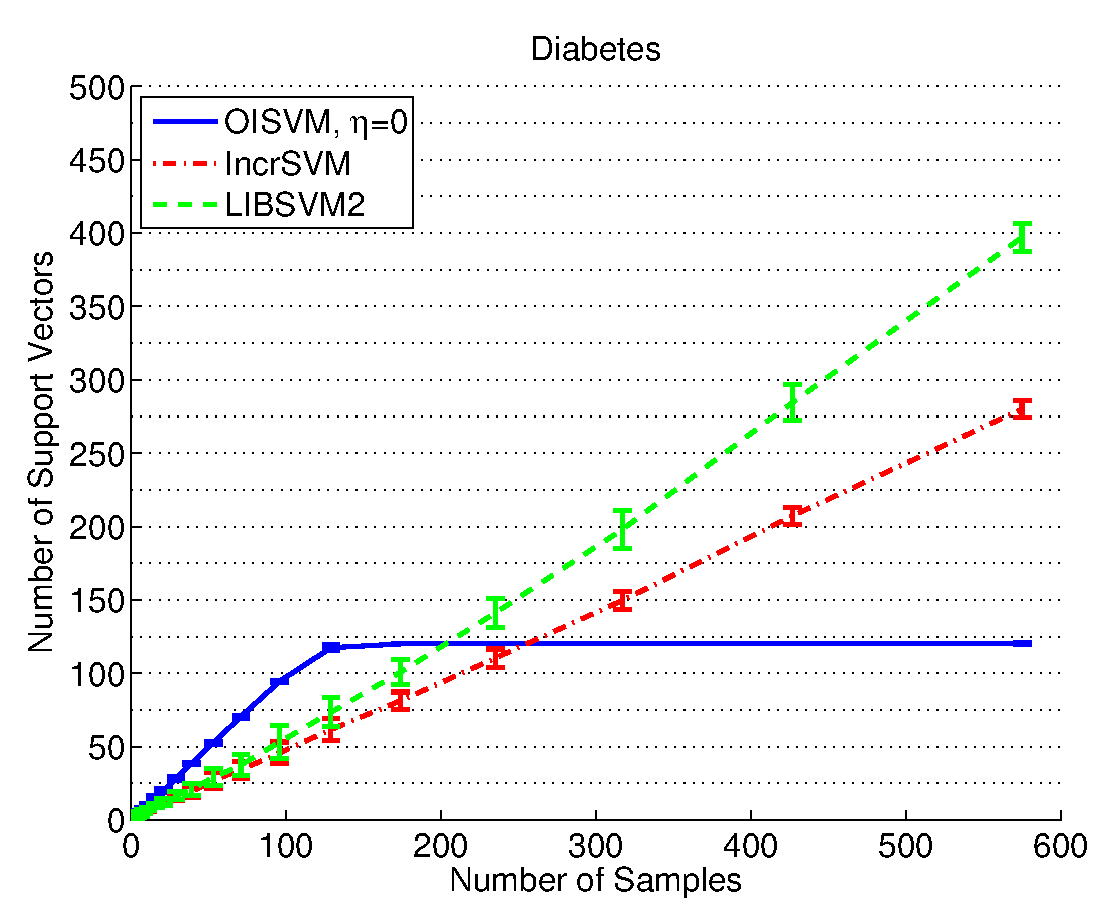
\includegraphics[width=0.48\linewidth]{figs/results/diabetis_sv} &
  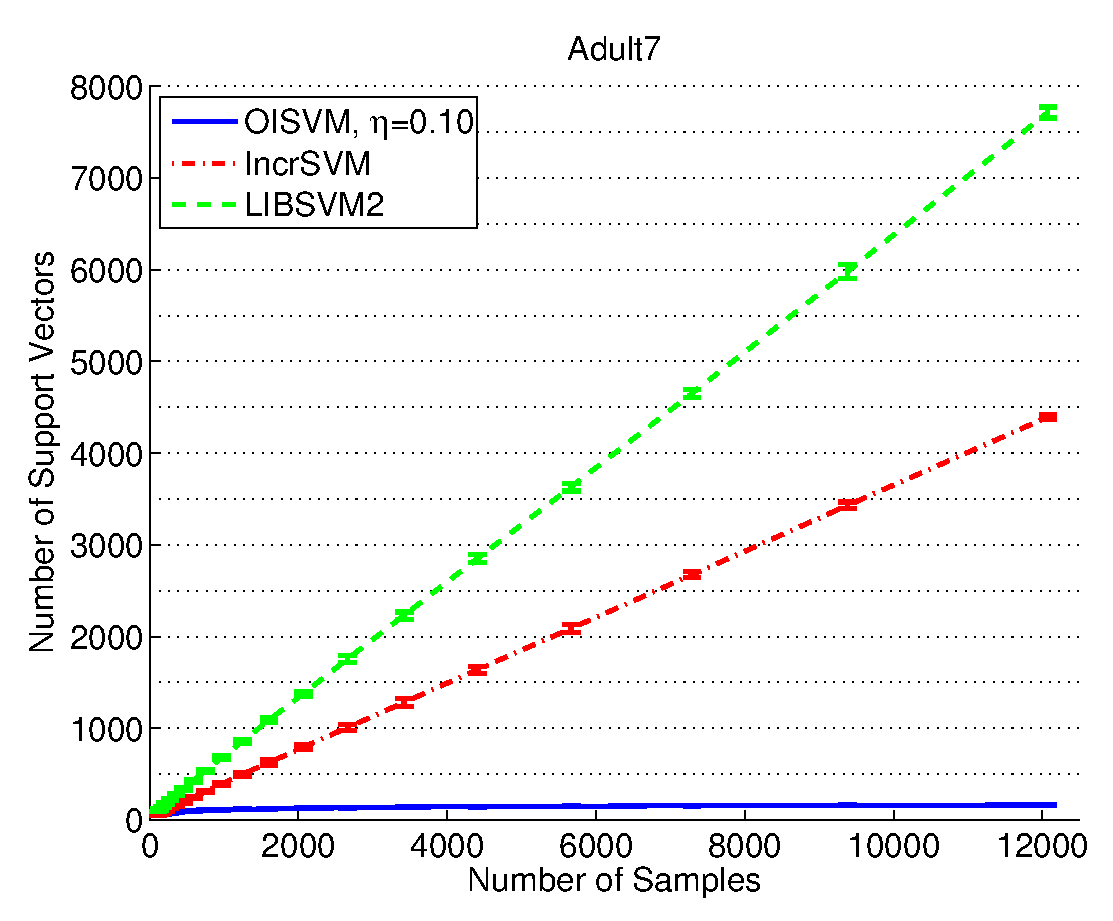
\includegraphics[width=0.48\linewidth]{figs/results/adult7_sv} 
  \end{tabular}
  \caption{Comparison of LIBSVM2, IncrSVM and OISVM and on the \emph{Diabetes}
  (left panel) and \emph{Adult7} (right panel) benchmarks.
  \emph{Diabetes} is solved using a polynomial kernel with degree $3$,
  while \emph{Adult7} is solved using a Gaussian kernel.}
\label{fig:ad7}
\end{figure*}

\begin{figure*}[t]
  \centering \footnotesize
  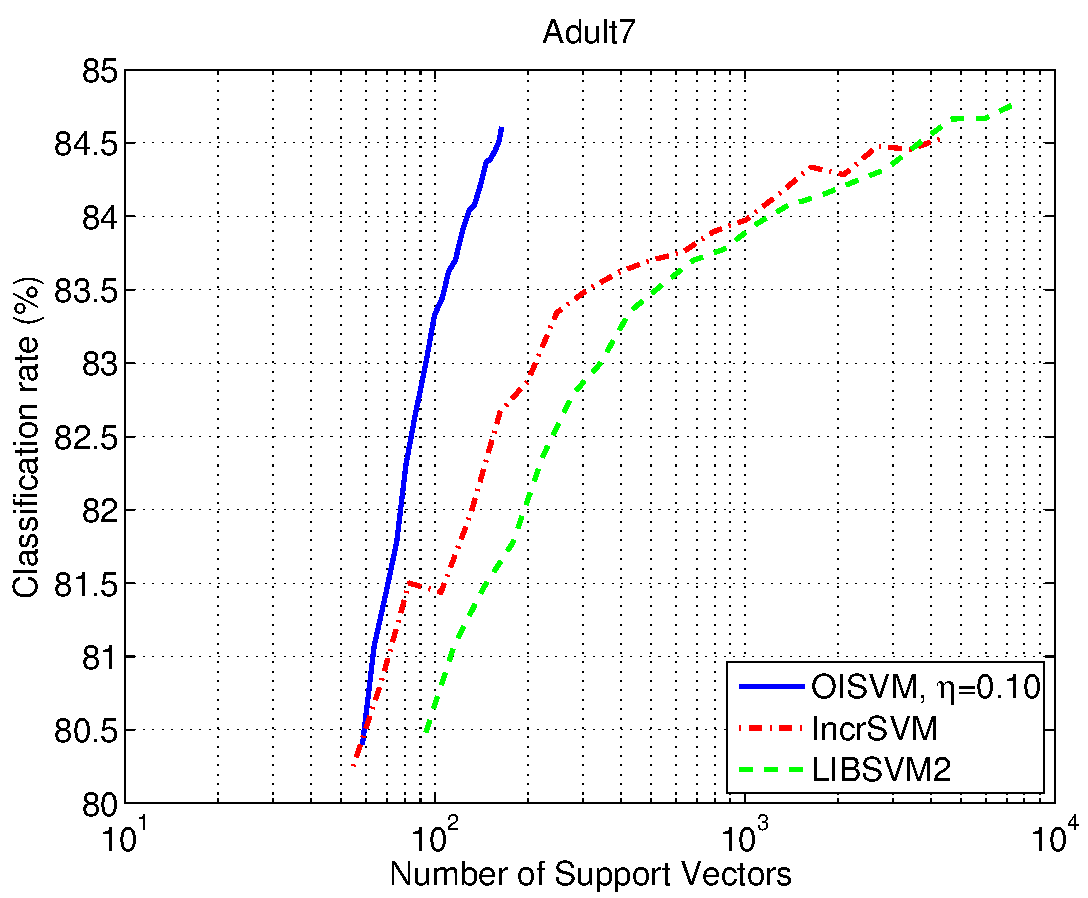
\includegraphics[width=0.48\linewidth]{figs/results/adult7_sv_cr}
  \caption{Comparison of LIBSVM2, IncrSVM and OISVM on the \emph{Adult7} dataset.}
\label{fig:sv_cr}
\end{figure*}

\begin{table}[t]
\tiny
\renewcommand{\arraystretch}{1.3}
\caption{Comparison of OISVM, RSVM, IncrSVM and LIBSVM2 on 10 standard benchmarks, solved
 using a Gaussian kernel. For each benchmark, we report the classification rate and
 the number of SVs. The value of $\eta$ has been chosen in order not to loose
 more than $0.5\%$ accuracy with respect to LIBSVM2.}
\label{table:t1}
\centering
\begin{tabular}[!h]{lcccc}
\hline
    Dataset   & OISVM                           & RSVM           & LIBSVM2                          & IncrSVM                            \\ \hline
     Banana   & $89.54\pm0.41$ ($18.90\pm1.29$) & $88.81\pm0.63$ & $89.75\pm0.30$ ($173.60\pm21.20$) & $89.77\pm0.28$ ($121.10\pm9.01$)  \\
     Breast   & $73.51\pm4.21$ ($36.00\pm2.67$) & $71.95\pm4.79$ & $74.03\pm4.15$ ($199.70\pm0.67$)  & $74.55\pm4.16$ ($122.60\pm4.95$)  \\
     Diabetis & $76.83\pm2.13$ ($8.60\pm0.52$)  & $75.77\pm2.85$ & $76.83\pm2.21$ ($417.00\pm4.00$)  & $76.83\pm1.77$ ($283.30\pm8.17$)  \\
     Flare    & $66.35\pm1.17$ ($10.40\pm0.70$) & $63.77\pm4.05$ & $66.35\pm1.23$ ($631.10\pm4.20$)  & $67.15\pm1.63$ ($555.70\pm8.59$)  \\
     German   & $76.20\pm1.93$ ($52.60\pm2.46$) & $75.43\pm2.20$ & $76.70\pm1.79$ ($600.70\pm11.89$) & $76.37\pm2.60$ ($384.70\pm7.01$)  \\
     Heart    & $84.90\pm1.91$ ($14.30\pm0.67$) & $84.30\pm2.95$ & $85.00\pm1.83$ ($161.60\pm2.63$)  & $85.00\pm2.87$ ($85.00\pm3.27$)   \\
     Ringnorm & $98.03\pm0.27$ ($87.60\pm6.01$) & $98.60\pm0.10$ & $98.57\pm0.10$ ($377.00\pm4.06$)  & $98.50\pm0.10$ ($213.00\pm4.74$)  \\
     Titanic  & $77.84\pm0.66$ ($11.90\pm1.37$) & $74.81\pm3.24$ & $77.60\pm1.63$ ($146.00\pm5.27$)  & $77.28\pm0.35$ ($86.80\pm6.91$)   \\
     Twonorm  & $97.14\pm0.34$ ($60.60\pm5.44$) & $97.18\pm0.32$ & $97.44\pm0.26$ ($400.00\pm0.00$)  & $97.65\pm0.09$ ($299.90\pm5.74$)  \\
     Waveform & $89.67\pm0.47$ ($78.20\pm3.12$) & $89.66\pm0.65$ & $90.10\pm0.36$ ($324.60\pm9.43$)  & $89.62\pm0.58$ ($220.30\pm10.49$) \\ \hline
\end{tabular}
\end{table}

For a complete comparison we have used also a variation of the Reduced
Support Vector Machine (RSVM) method \cite{LeeM01}, the same used also
in \cite{KeerthiCDC06}, in which for each run we have randomly
selected a number of basis vectors equal to the one selected by
OISVM. In this way we compare the two methods with the same number
of basis vectors. We have used a Wilcoxon signed-ranks test to compare the
performances of the two methods, as suggested in \cite{Demsar06},
obtaining a p-value less than $0.02$. This confirms that our strategy
to select basis vectors is better than the random sampling,
suggested by many authors, e.g. \cite{RifkinYP03}. As a plus our
strategy assures that, as said before, the growth of basis vectors
will always eventually stop.

To gain more understanding on the difference between RSVM and OISVM we
have also compared the value of the objective function
(\ref{eqn:svm_primal}) at the end of each dataset. The results are in
Table \ref{table:t1_o}, where the relative difference between the
value of the objective function of OISVM and RSVM compared to LIBSVM2
are shown. There is a clear correlation between good classification
accuracy and good value of the objective function. Hence our method
seems to select the basis vectors in a way that allows a better
minimization of (\ref{eqn:svm_primal}). This can be explained
intuitively noting that adding a linearly dependent vector to the basis
set will not help in minimizing the objective function.
The negative result on \emph{Ringnorm} is somehow surprising given the corresponding
good classification performance, but it should not worry as
the value of the objective function is loosely related to the classification performance.
Hence the big increment in the objective function does not necessarily
correspond to very bad classification performance, as it is shown
in Table \ref{table:t1}.

We have also conducted other experiments to compare the speed of the
algorithms. Given that our implementation is in Matlab, so not optimized for
speed, to have a fair comparison we have considered the number of kernel
evaluations as a figure of merit. This is a standard measure
for an implementation invariant comparison\footnote{However note that our Matlab implementation
of OISVM is about 1 order of magnitude faster than the Matlab implementation of IncrSVM.},
see for example \cite{BordesEWB05,DiehlC03}.
We have used 3 databases, \emph{Adult7}, \emph{Banana} and \emph{Waveform}, with
the same kernel and parameters used in \cite{BordesEWB05}. 
In Fig. \ref{fig:kernel_eval} we show the performance on the test set
as a function of the number of kernel evaluations. For LIBSVM2 and IncrSVM we have just
a point on the graph, while for OISVM we have a curve obtained varying $\eta$\footnote{
The values of $\eta$ for the 3 datasets are respectively $[0.4;0.3;0.2;0.1;0.05;0.01],
[0.7;0.6;0.5;0.4;0.3;0.2;0.1;0.01],[0.8;0.7;0.6;0.5;0.4;0.3]$.}.
In other words, in OISVM we can trade accuracy for training (and testing) speed.
From the figure we can see that OISVM achieves better or comparable performance
to the other methods with much less kernel computations. Moreover the degree of freedom
given by the sparsification method allows to trade just 0.5\% of performance to
save more than 1 order of magnitude of kernel computations.
Note that the accuracy of OISVM is not always monotonically increasing with
$\eta$ going to 0. A possible explanation is that the sparsification procedure
can be seen as a form of regularization; a similar view has been proposed in 
\cite{BlanchardMVZ05}. Hence it is plausible to suppose that there is an optimal
value of $\eta$ that gives better generalization properties.

\begin{table}
%\renewcommand{\arraystretch}{1.3}
\caption{Loss in percentage of the objective function of OISVM and RSVM in relation to the one
 of LIBSVM2 on 10 standard benchmarks, solved using a Gaussian kernel. The values of $\eta$
 are the same of Table \ref{table:t1}.}
\label{table:t1_o}
\centering
\footnotesize
\begin{tabular}[!h]{lcccc}
\hline
    Dataset   & OISVM          & RSVM            \\ \hline
     Banana   & $13.9\pm3.2$ & $23.5\pm10.5$ \\
     Breast   & $2.1\pm0.4$  & $3.3\pm0.4$   \\
     Diabetis & $1.7\pm1.2$  & $3.8\pm4.7$   \\
     Flare    & $0.1\pm0$    & $4.6\pm6.3$   \\
     German   & $9.7\pm1.4$  & $9.9\pm0.5$   \\
     Heart    & $0.9\pm0.3$  & $1.5\pm1.0$   \\
     Ringnorm & $43.0\pm4.6$ & $3.6\pm0.4$   \\
     Titanic  & $0\pm0$      & $15.8\pm10.8$ \\
     Twonorm  & $5.6\pm0.8$  & $8.9\pm1.0$   \\
     Waveform & $10.4\pm0.6$ & $10.4\pm1.0$  \\ \hline
\end{tabular}
\end{table}

\begin{figure*}[!ht]
  \centering \footnotesize
  \begin{tabular}{cc}
  \multicolumn{2}{c}{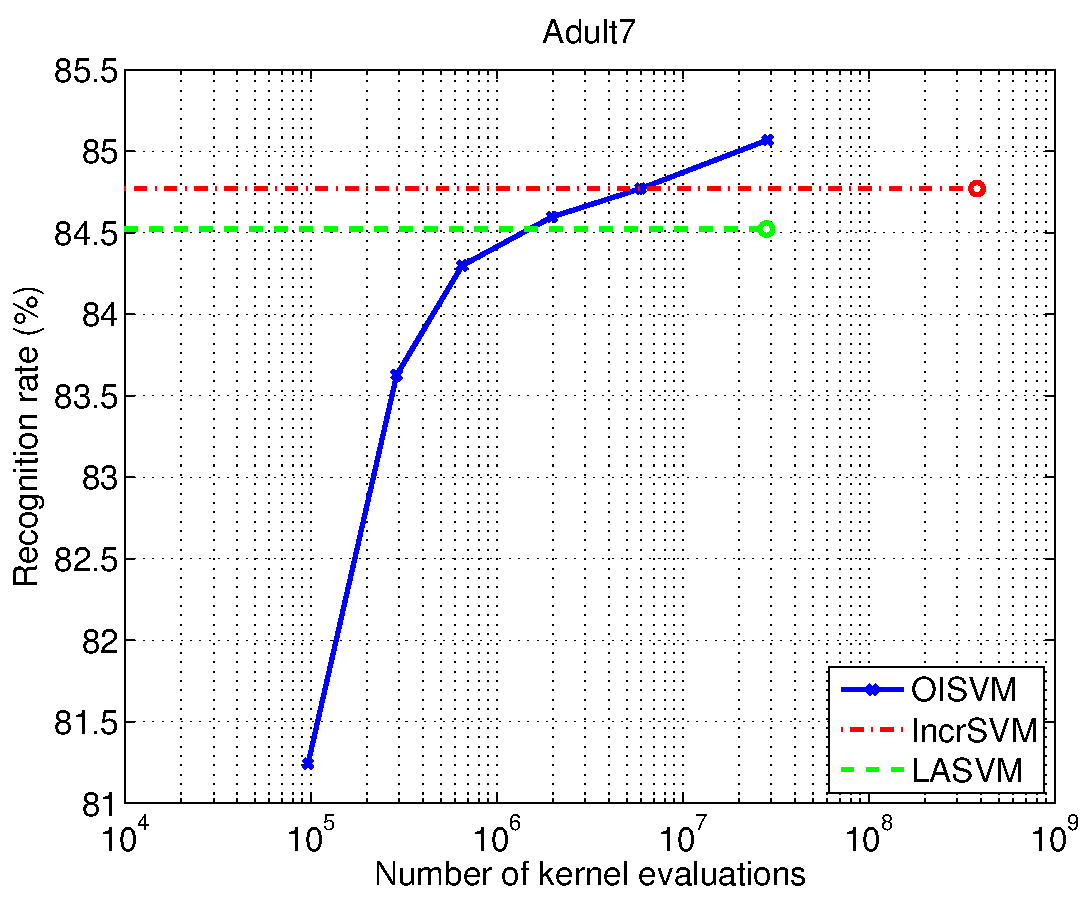
\includegraphics[width=0.48\linewidth]{figs/results/fig_a7a}} \\
  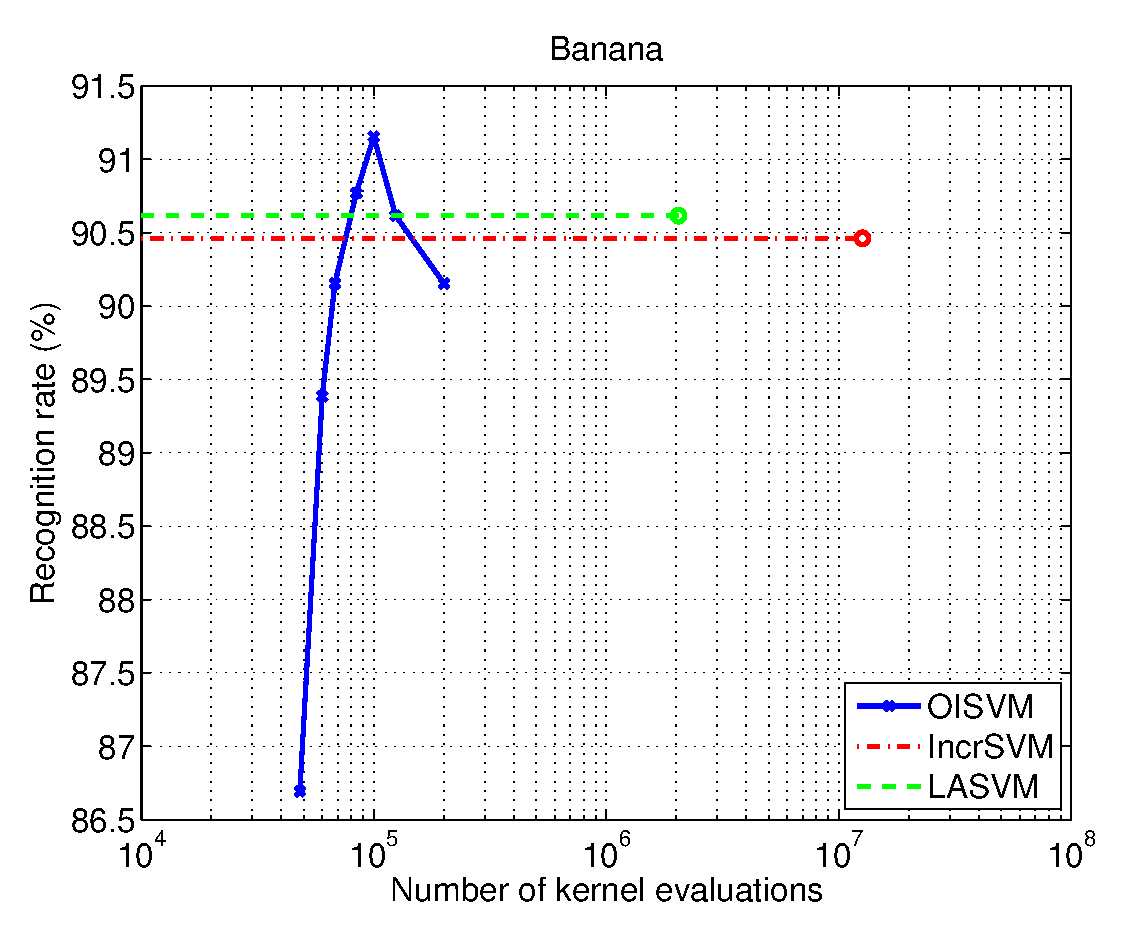
\includegraphics[width=0.48\linewidth]{figs/results/fig_banana} &
  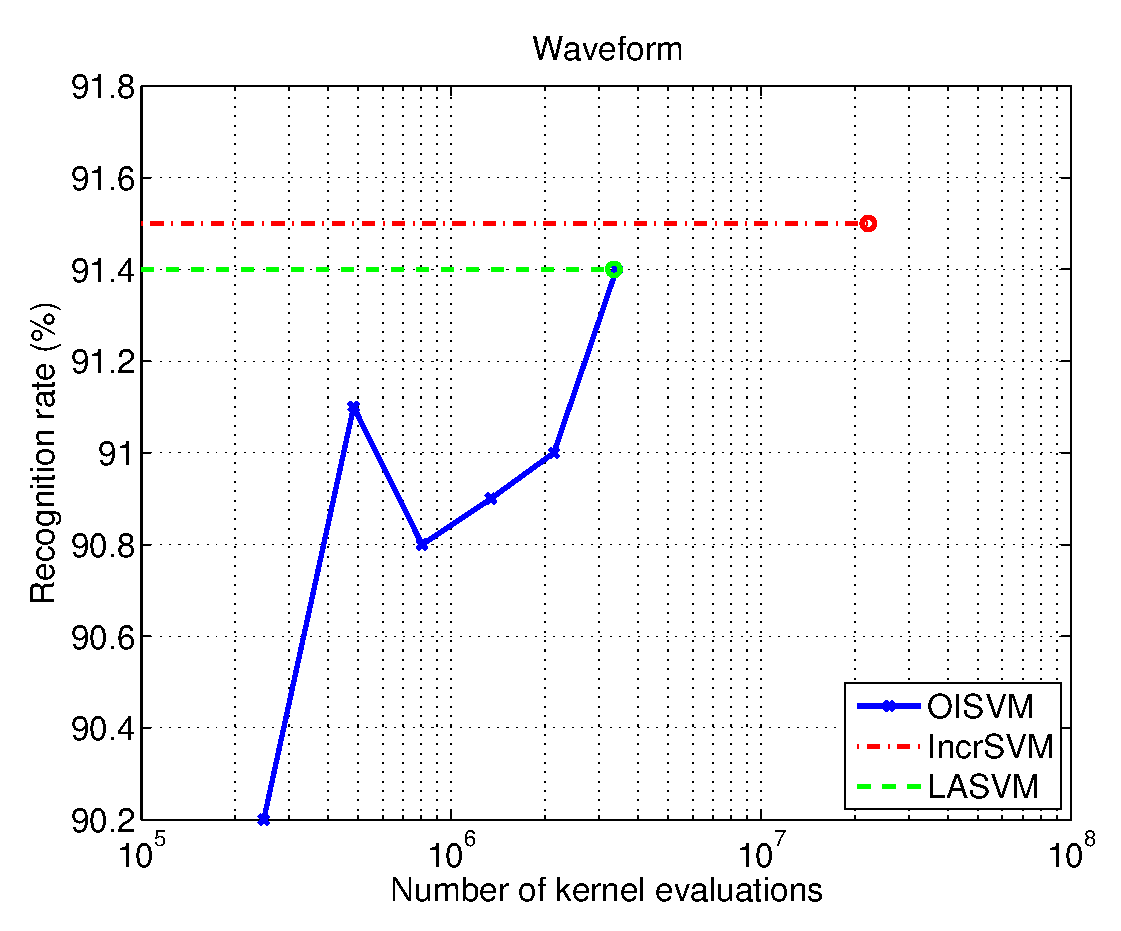
\includegraphics[width=0.48\linewidth]{figs/results/fig_waveform}
  \end{tabular}
  \caption{Trade-off between accuracy and number of kernel evaluations of OISVM, IncrSVM and
  LASVM on 3 benchmarks.
  The OISVM curve is obtained plotting the number of kernel evaluations and the recognition rate at the end of the training, for each value of $\eta$. The number of kernel evaluations increases as $\eta$ decreases. 
  In LASVM and IncrSVM there is no parameter to trade accuracy for training speed, so only one
  point is shown.}
\label{fig:kernel_eval}
\end{figure*}


\subsection{Robot Navigation}
\label{sec:exp2}
We performed a second series of experiments, namely place recognition
in an indoor environment, to evaluate our algorithm. We considered a
realistic scenario where the algorithm had to incrementally update the
model, so to adapt to the variations in an indoor environment due to
human activities over long time spans. These variations include people
appearing in different rooms during working time, objects such as cups
moved or taken in/out of the drawers, pieces of furniture pushed
around, and so forth.

\begin{figure*}[t]
\centering \footnotesize
\begin{tabular}{@{}c@{\hspace{0.002\linewidth}}c@{\hspace{0.002\linewidth}}
c@{\hspace{0.002\linewidth}}c@{\hspace{0.002\linewidth}}
c@{\hspace{0.002\linewidth}}c@{\hspace{0.002\linewidth}}
c@{\hspace{0.002\linewidth}}c@{}}
% -------------------------------------------------------------------
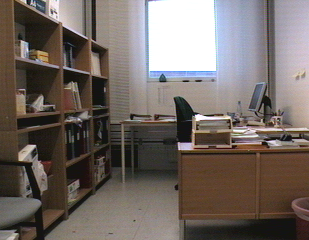
\includegraphics[width=0.123\linewidth]{figs/idol/bo_cloudy.png} &
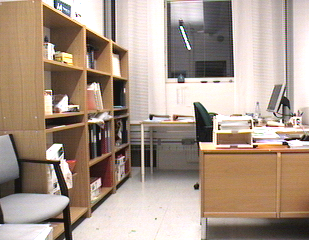
\includegraphics[width=0.123\linewidth]{figs/idol/bo_night.png}  &
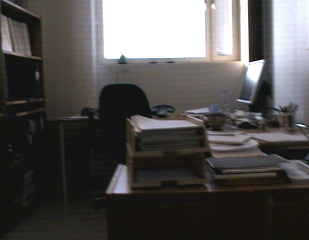
\includegraphics[width=0.123\linewidth]{figs/idol/bo_sunny.png}  &
\includegraphics[width=0.123\linewidth]{figs/idol/cr_cloudy.png} &
\includegraphics[width=0.123\linewidth]{figs/idol/cr_night.png}  &
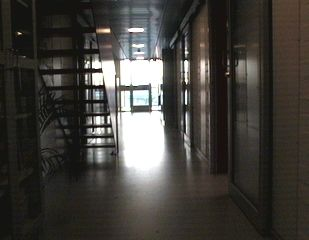
\includegraphics[width=0.123\linewidth]{figs/idol/cr_sunny.png} &
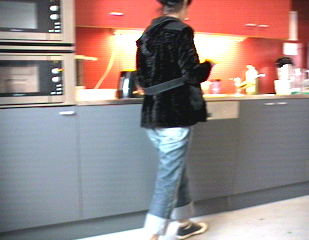
\includegraphics[width=0.123\linewidth]{figs/idol/people1.png}  &
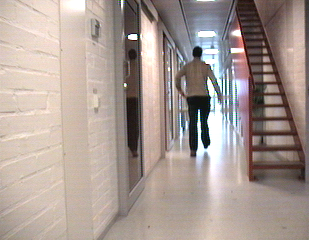
\includegraphics[width=0.123\linewidth]{figs/idol/people2.png}  \\
% -------------------------------------------------------------------
\includegraphics[width=0.123\linewidth]{figs/idol/cup1.png}   &
\includegraphics[width=0.123\linewidth]{figs/idol/cup3.png}   &
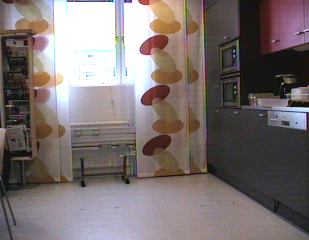
\includegraphics[width=0.123\linewidth]{figs/idol/chair1.png}   &
\includegraphics[width=0.123\linewidth]{figs/idol/chair3.png} &
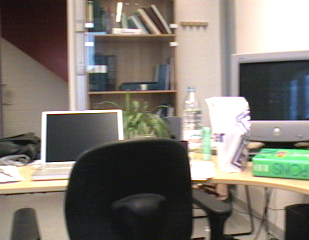
\includegraphics[width=0.123\linewidth]{figs/idol/time1.png} &
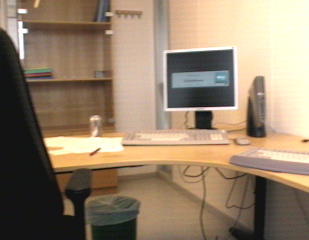
\includegraphics[width=0.123\linewidth]{figs/idol/time2.png} &
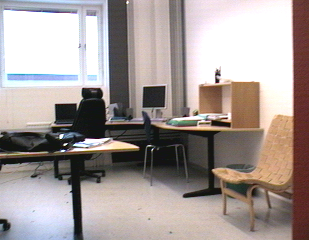
\includegraphics[width=0.123\linewidth]{figs/idol/time3.png}  &
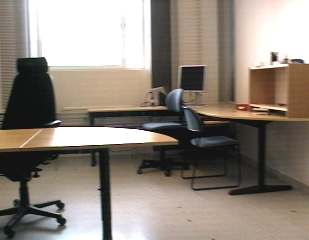
\includegraphics[width=0.123\linewidth]{figs/idol/time4.png}  \\
% -------------------------------------------------------------------

\includegraphics[width=0.123\linewidth]{figs/idol/drive1.png}   &
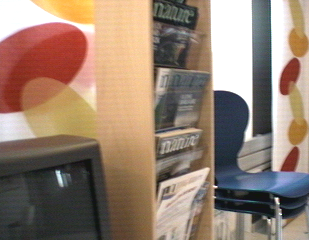
\includegraphics[width=0.123\linewidth]{figs/idol/drive2.png}   &
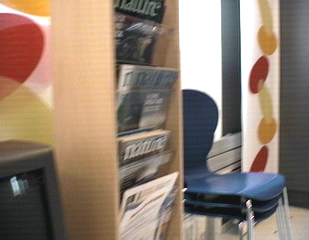
\includegraphics[width=0.123\linewidth]{figs/idol/drive3.png}   &
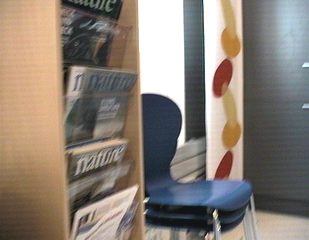
\includegraphics[width=0.123\linewidth]{figs/idol/drive4.png} &
\includegraphics[width=0.123\linewidth]{figs/idol/drive5.png} &
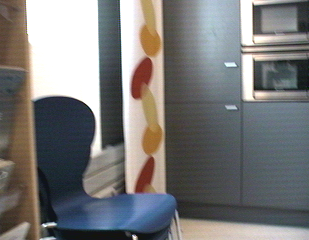
\includegraphics[width=0.123\linewidth]{figs/idol/drive6.png} &
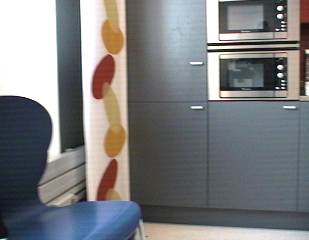
\includegraphics[width=0.123\linewidth]{figs/idol/drive7.png}  &
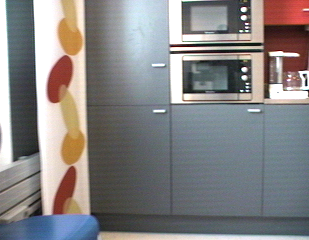
\includegraphics[width=0.123\linewidth]{figs/idol/drive8.png}   \\
% -------------------------------------------------------------------
\end{tabular}
\caption{Sample images illustrating the variations captured in the IDOL2 database.
Images in the top row show the variability introduced by changes in
illumination for two rooms (first six images) as well as people
appearing in the environment.  The middle row shows the influence of
people's everyday activity (first four images) as well as larger
variations which happened over a time span of $6$ months. Finally, the
bottom row illustrates the changes in viewpoint observed for a series
of images acquired one after another in $1.6$ seconds.}
\label{fig:idol}
\end{figure*}

Experiments were conducted on the IDOL2 database (Image Database for
rObot Localization 2, \cite{luo:idol2}), which contains $24$ image
sequences acquired using a perspective camera mounted on two mobile
robot platforms. The acquisition was performed within an indoor
laboratory environment consisting of five rooms of different
functionality. The sequences were acquired under various weather and
illumination conditions (sunny, cloudy, and night) and across a time
span of six months. Thus, these data capture natural variability that
occurs in real-world environments because of both natural changes in
the illumination and human activity. Fig. \ref{fig:idol} shows some
sample images from the database, illustrating the difficulties of the
task.  The image sequences in the database are divided as follows: for
each robot platform and for each type of illumination conditions,
there were four sequences recorded. Of these four sequences, the first
two were acquired six months before the last two. This means that, for
each robot and for every illumination condition, there are always two
sequences acquired under similar conditions, and two sequences
acquired under very different conditions. This makes the database
suitable for different kinds of evaluation on the adaptability of an
incremental algorithm. For further details about the database, we
refer the readers to \cite{luo:idol2}.

The evaluation was performed using composed receptive field histograms
(CRFH) \cite{linde:icpr04} as global image features and SIFT
\cite{Lowe99} for extracting local features. In the experiments, we
consider both the \emph{exponential $\chi^2$} kernel for SVM (when
using CRFH), and the \emph{matching kernel} \cite{WallravenCG03} (when
using SIFT). Note that the kernel in \cite{WallravenCG03} is not
always positive semidefinite \cite{BoughorbelTF04}, so this is also a
test on non-Mercer kernels that have proved useful for visual
recognition. The kernels used are infinite-dimensional, so for both
kernels we run the OISVM using different values of $\eta$.

We benchmarked OISVM against the approximate incremental SVM
extension of fixed-partition technique \cite{SyedLS99} and 
the IncrSVM algorithm. The algorithms were trained incrementally on
three sequences from IDOL2, acquired under similar illumination
conditions with the same robot platform; the fourth sequence was used
for testing. In order to test the various properties of interest of
the incremental algorithms, we need a reasonable number of incremental
steps. Thus, every sequence was split into $5$ subsequences, so that
each subset contained one of the five images acquired by the robot
every second (image sequences were acquired at a rate of
$5$fps). Since during acquisition the camera's viewpoint continuously
changes \cite{luo:icra07}, the subsequences could be considered as
recorded separately in a static environment but for varying pose.
This setup allows us to examine how the algorithms perform on data
with less variations. In order to get a feeling of the variations of
the frame images in a sequence, the bottom row of Fig. \ref{fig:idol}
shows some sample images acquired within a time span of $1.6$
sec. As a result, training on each sequence was
performed in $5$ steps, using one subsequence at a time, resulting in
$15$ steps in total. Overall, we considered $36$ different
permutations of training and test sequences for the exponential
$\chi^2$ kernel and for the matching kernel; here we report the
average results, plus/minus one standard deviation.
Fig. \ref{fig:exp:idol}, left, shows the recognition rates of the
exponential $\chi^2$ kernel (top) and matching kernel (bottom)
experiments obtained at each step using OISVM, IncrSVM and the
approximate incremental algorithm. Fig. \ref{fig:exp:idol}, right,
reports the number of support vectors stored in the model at each step
of the incremental procedure, for both kernel types.

We see that, performance-wise, all methods achieve statistically
comparable results; this is true for both kernel types. As far as the
machine size is concerned, the OISVM algorithm shows a considerable
advantage with respect to the fixed-partition method and IncrSVM. In the case of
the exponential $\chi^{2}$ kernel this advantage is truly impressive
(Fig \ref{fig:exp:idol}, top right): for $\eta=0.017$ and $0.025$ the
size at the final incremental step is $34\%/22\%$ of that of the
fixed-partition method and $28\%/18\%$ of that of IncrSVM.
Even more important, OISVM, for these two values of $\eta$,
has found a plateau in memory, while for other methods the trend seems
to be of a growth proportional to the number of training data. Note
that the choice of the parameter $\eta$ is crucial for achieving an
optimal trade-off between compactness of the solution and optimal
performance.

It is very interesting to note that, in the case of the matching
kernel, the memory reduction for OISVM is less pronounced, and there
is no clear plateau in memory growth by any of the algorithms.  This
behavior might be due to several factors: to begin with, the matching
kernel is not a Mercer kernel \cite{BoughorbelTF04}; moreover, in the
induced space of the matching kernel, there seems to be a high
probability that pairs of training points be (almost) orthogonal to
each other (note that, as the kernel is not a Mercer one, the
geometric interpretation might not be valid). Anyway, given enough
training points, the machine will always reach a maximum size and will
stop growing \cite{EngelMM04}.

%% We can conclude that these results are in agreement with those
%% obtained on the machine learning benchmark databases, and show the
%% effectiveness of OISVM in controlling the growth of the SV solution
%% in this on-line learning scenario.

\begin{figure*}[t]
  \centering \footnotesize
  \begin{tabular}{c@{\hspace{0.5cm}}c}
  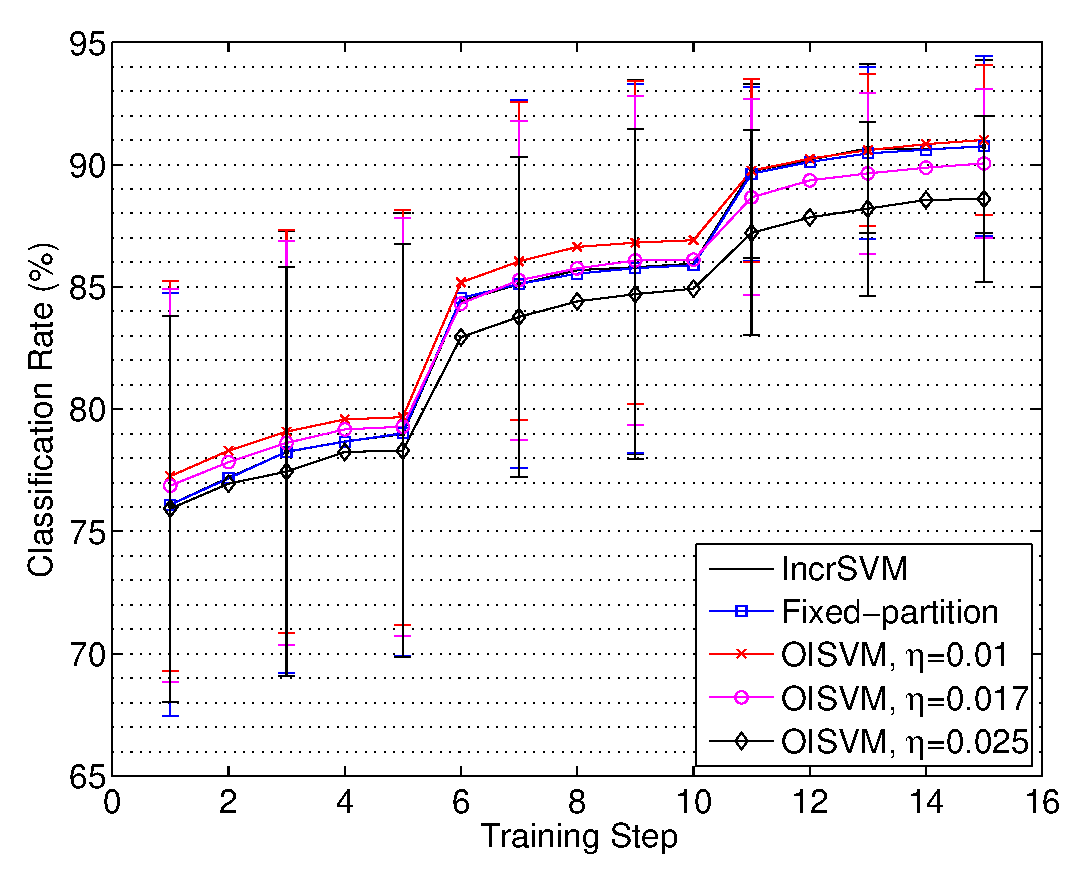
\includegraphics[width=0.47\linewidth]{figs/results/chi_cr} & 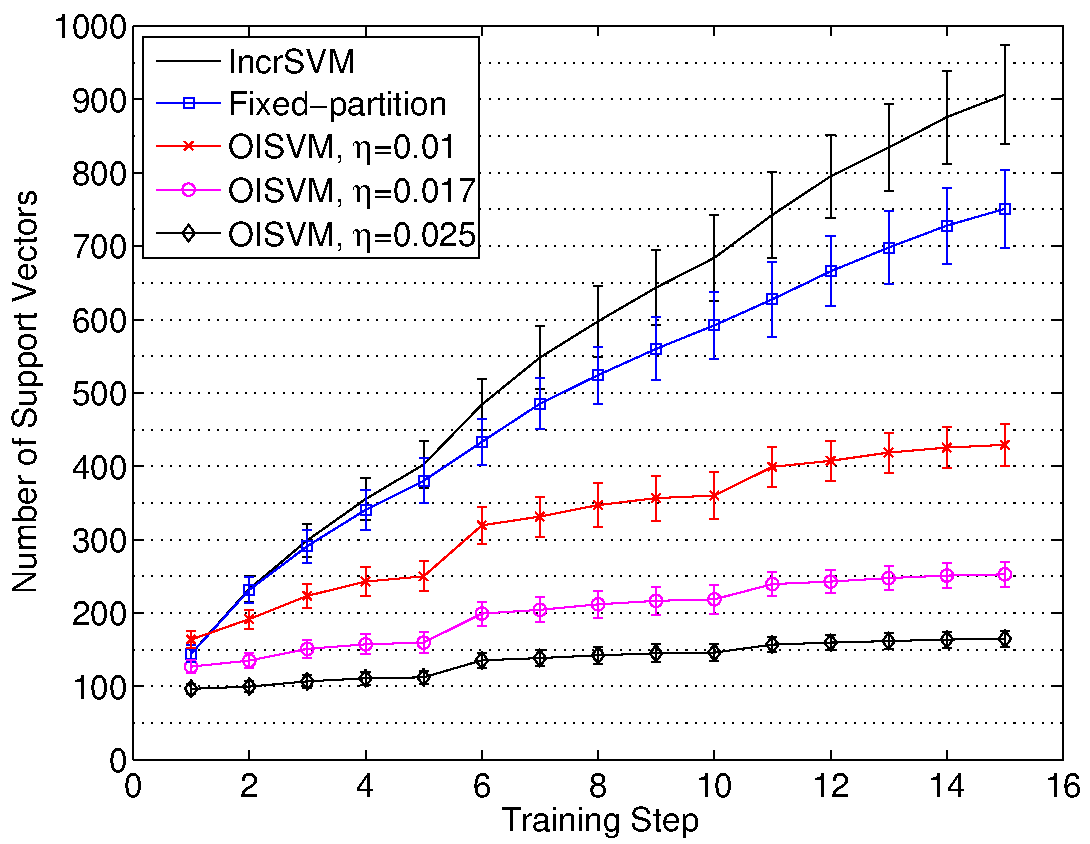
\includegraphics[width=0.47\linewidth]{figs/results/chi_sv}\\
  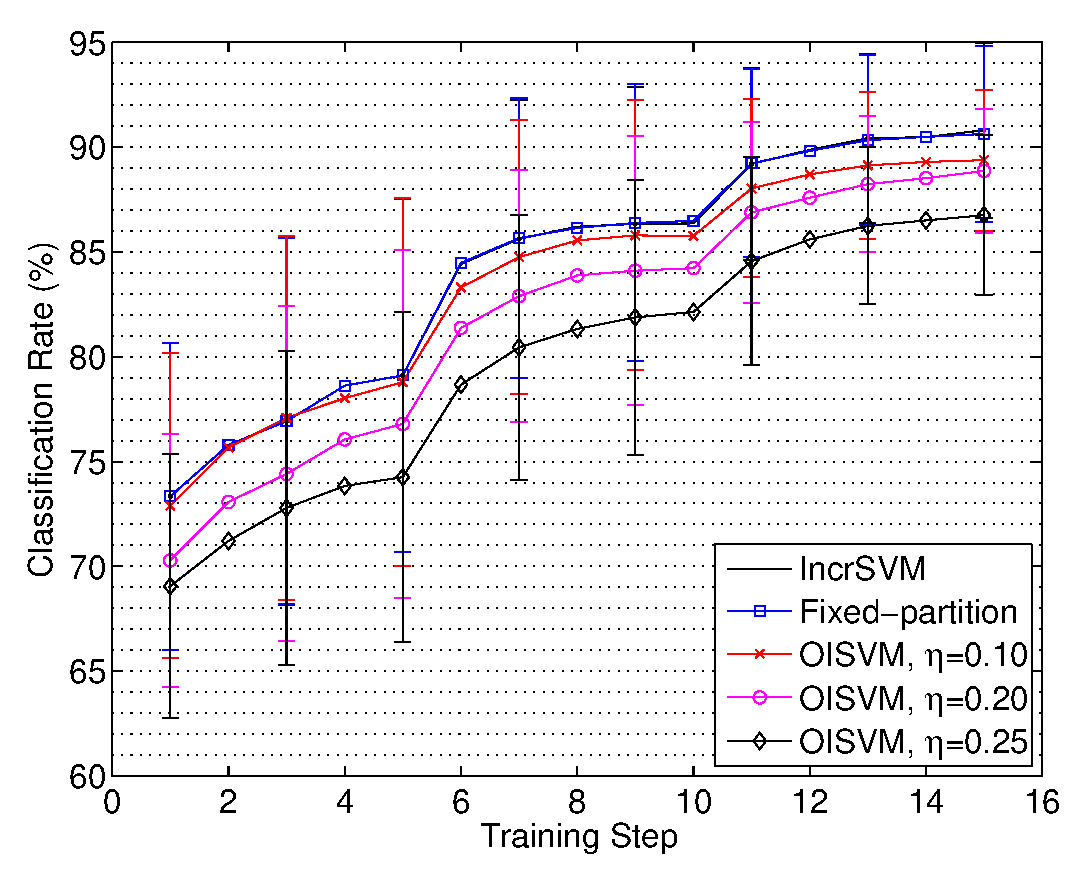
\includegraphics[width=0.47\linewidth]{figs/results/local_cr} & 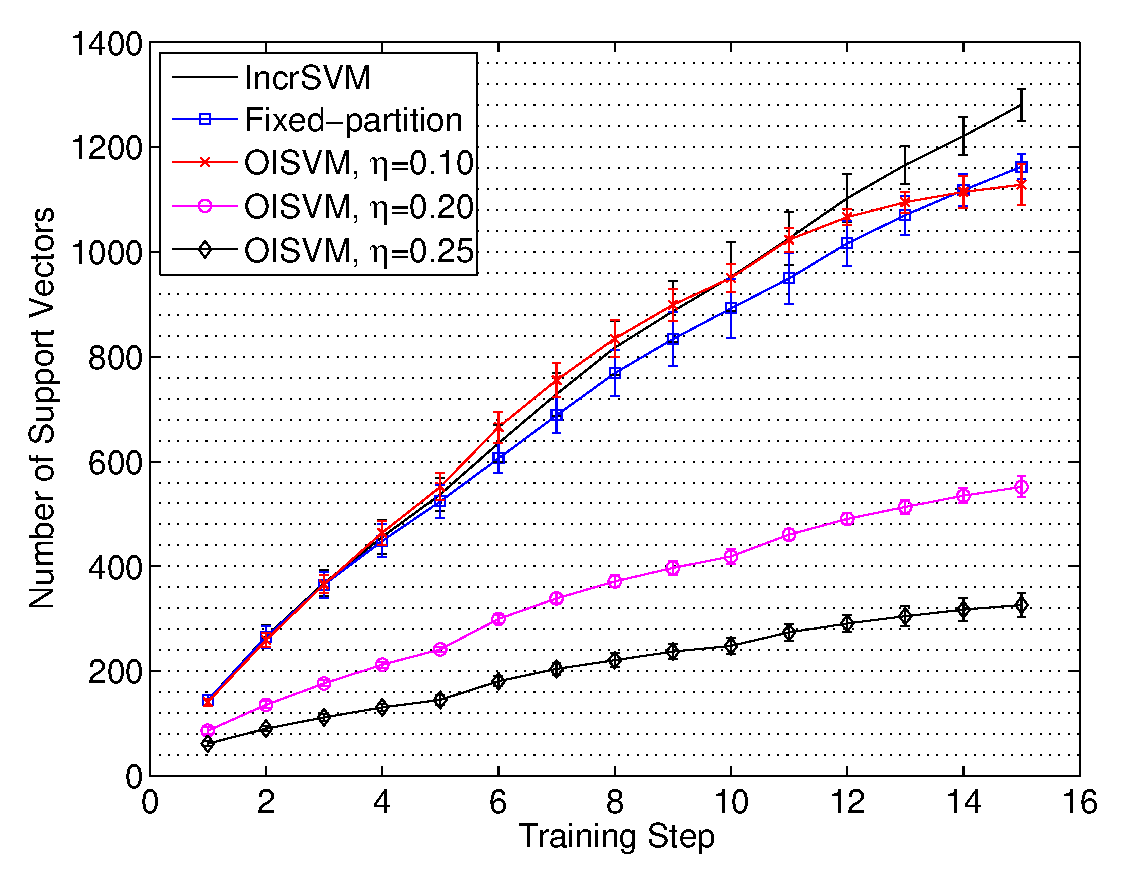
\includegraphics[width=0.47\linewidth]{figs/results/local_sv}\\
  \end{tabular}
\caption{Experimental results on the IDOL2 database, using OISVM with three
  different values of $\eta$, the fixed-partition and IncrSVM.
  Top: $\chi^2$ kernel, Bottom: matching kernel.}
\label{fig:exp:idol}
\end{figure*}


\subsection{Grasp Classification}
\label{sec:exp3}
In the third experiment, human subjects are involved in a grasping
task, which our system must identify; in particular, we are interested
in classifying the grasping posture independently of the subject and
the object being grasped.
%, thus focusing on the \emph{affordances} \cite{gibson} associated with objects.
Eight subjects were involved in
the experiment, $5$ men and $3$ women, all able-bodied, aged between
$23$ and $36$. They were given no prior knowledge on the aim and scope
of the experiment. Each subject would sit comfortably in front of a
workspace large about one squared meter and wear a $22$-sensors
Immersion CyberGlove \cite{cyberglove} on the right hand, and a Force
Resistor Sensor (FSR) on the thumb. Figure \ref{fig:devices} (upper
row) shows the devices, as worn by a subject.

\begin{figure*}[!ht]
  \begin{center}
    \begin{tabular}{c}
      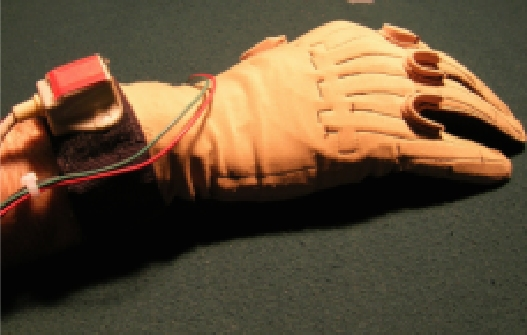
\includegraphics[height=0.08\textheight]{figs/grasping/devices1.jpg}
      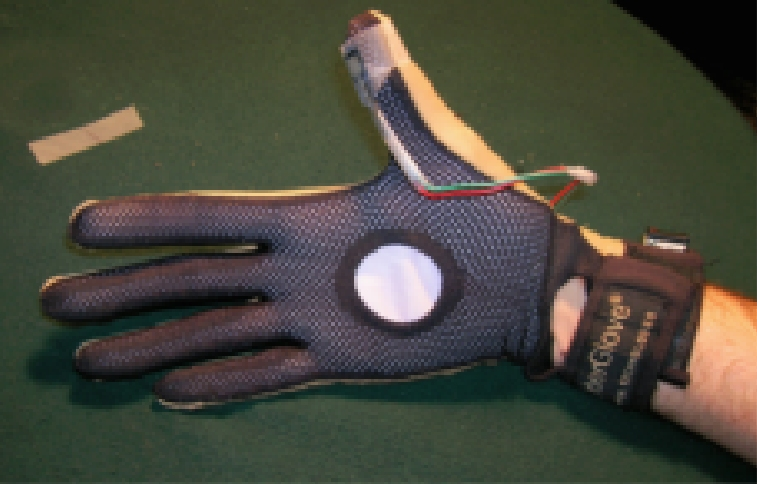
\includegraphics[height=0.08\textheight]{figs/grasping/devices2.jpg}
      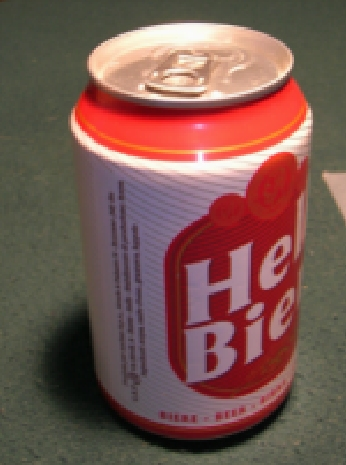
\includegraphics[height=0.08\textheight]{figs/grasping/beer.jpg}
      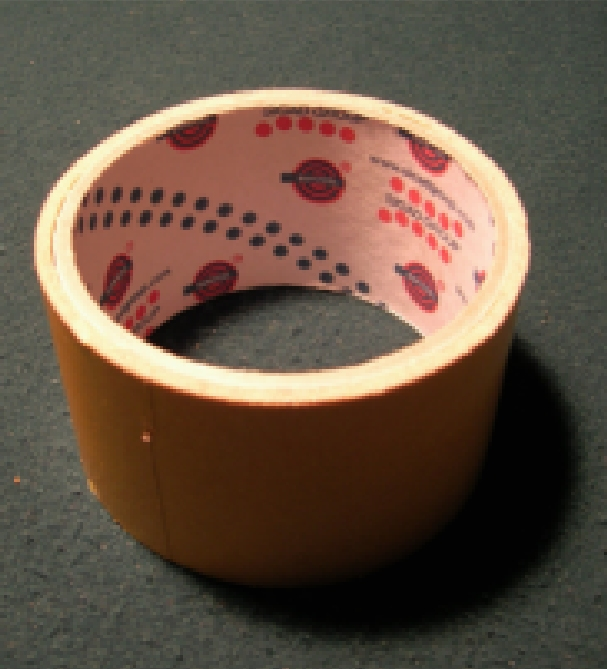
\includegraphics[height=0.08\textheight]{figs/grasping/scotch.jpg}
      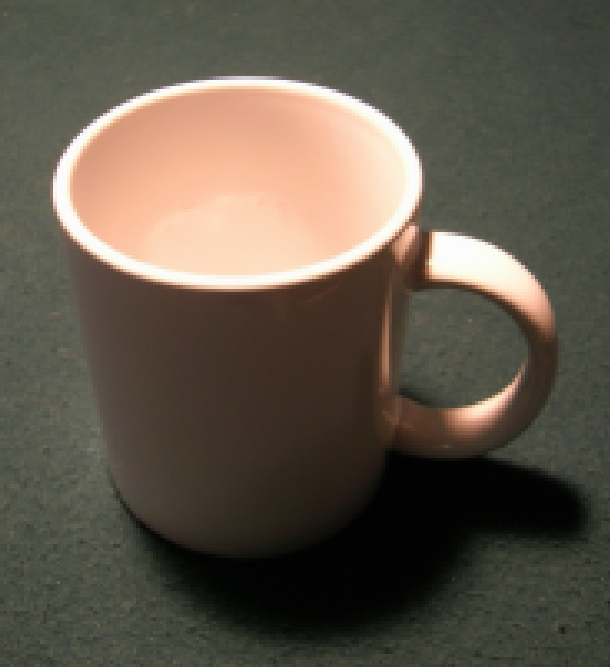
\includegraphics[height=0.08\textheight]{figs/grasping/mug.jpg} \\
      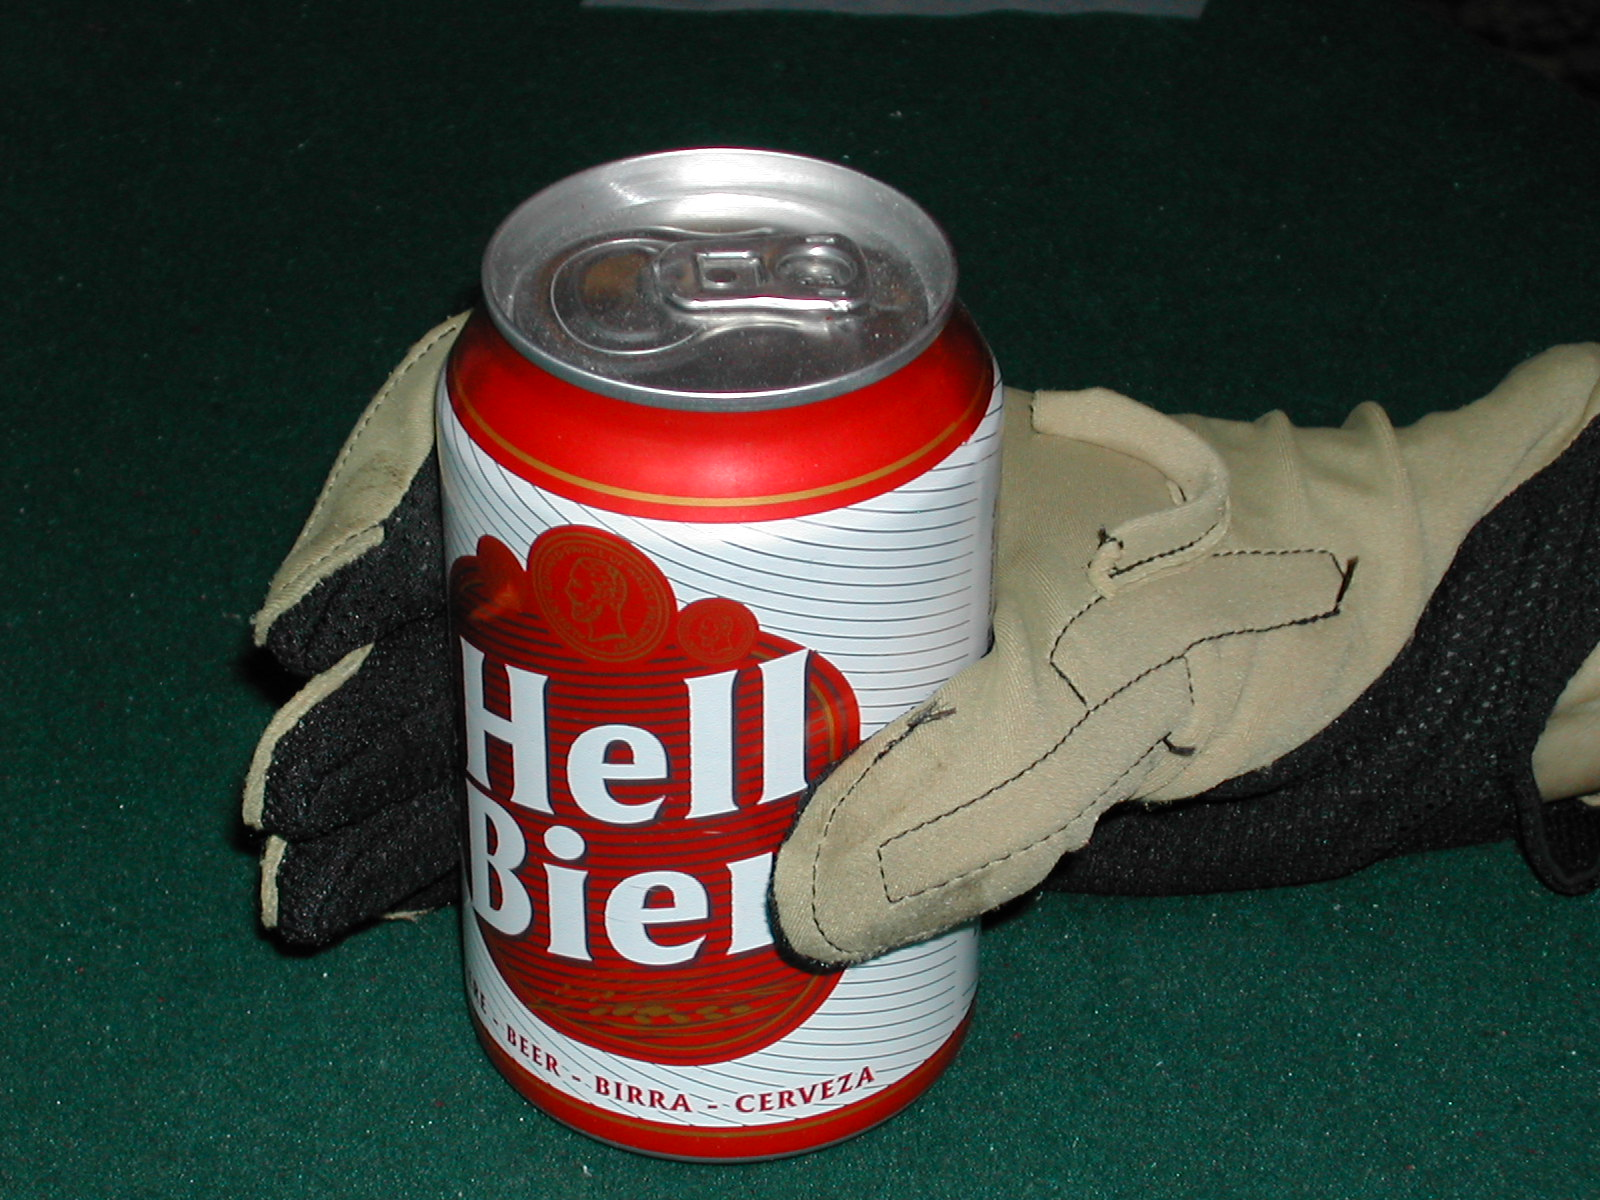
\includegraphics[height=0.08\textheight]{figs/grasping/grasp1.jpg}
      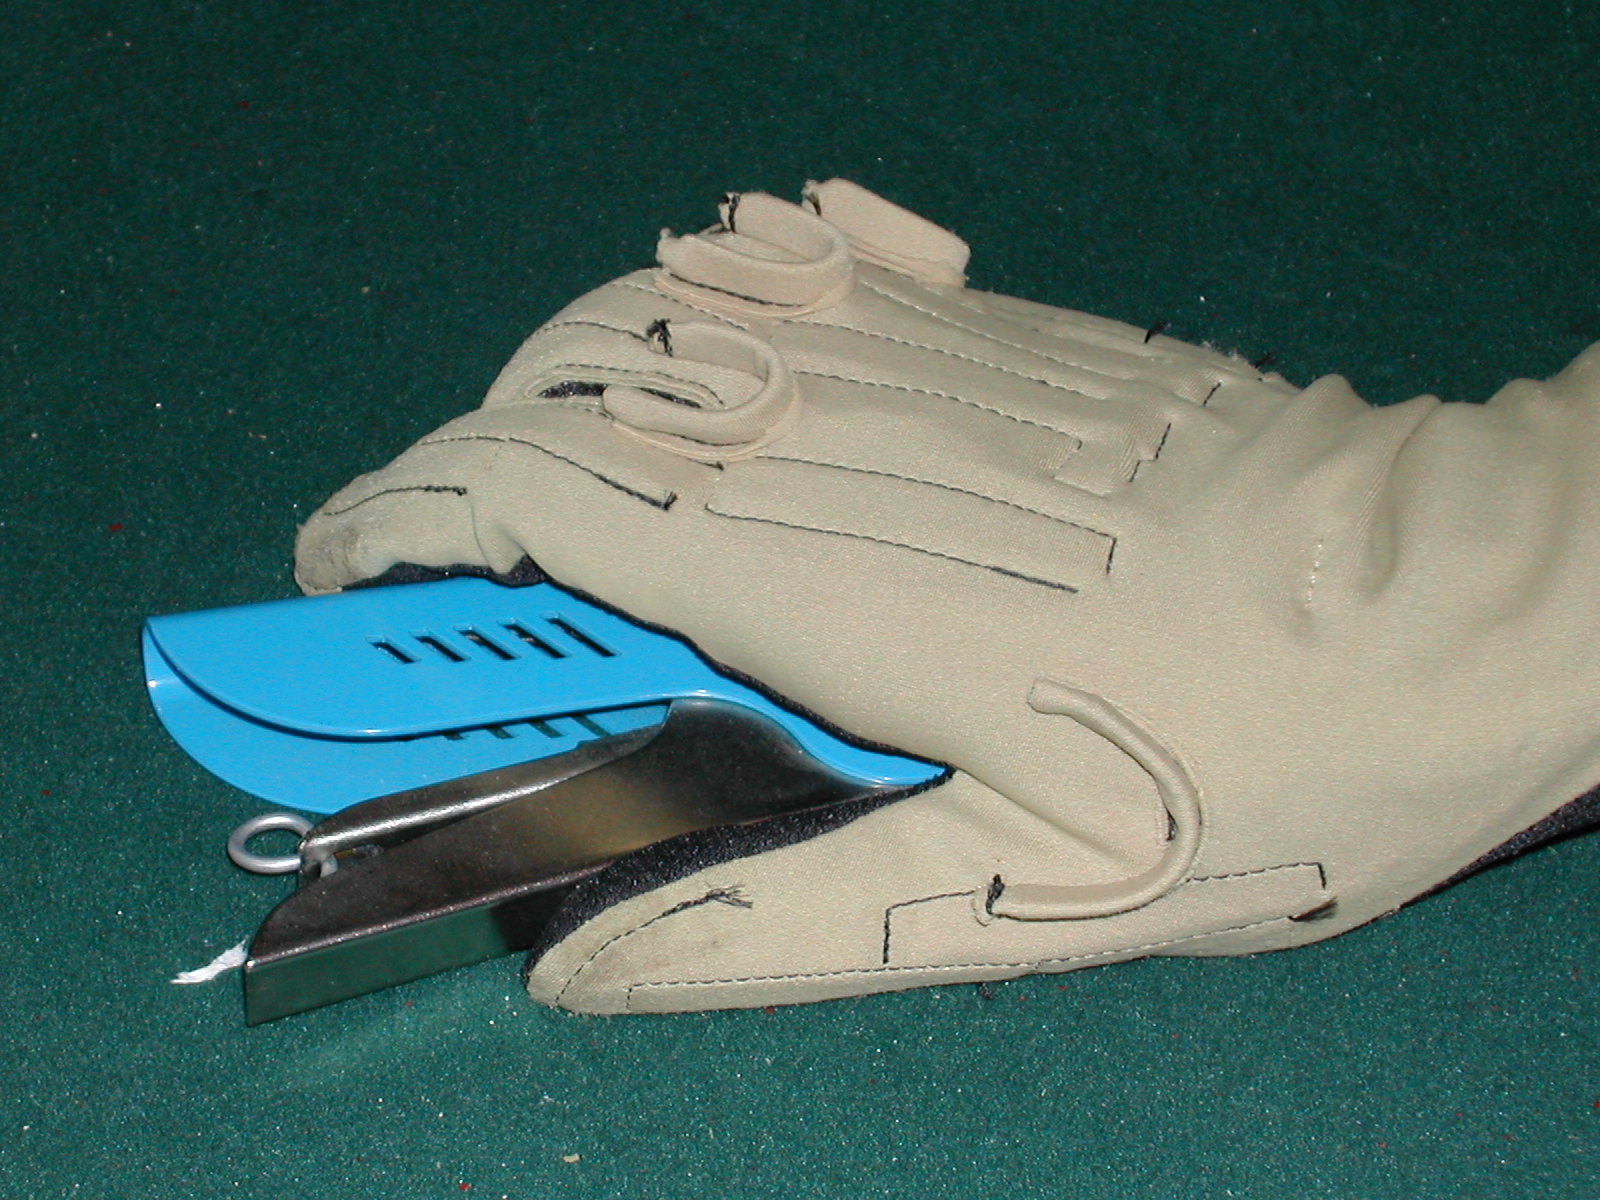
\includegraphics[height=0.08\textheight]{figs/grasping/grasp2.jpg}
      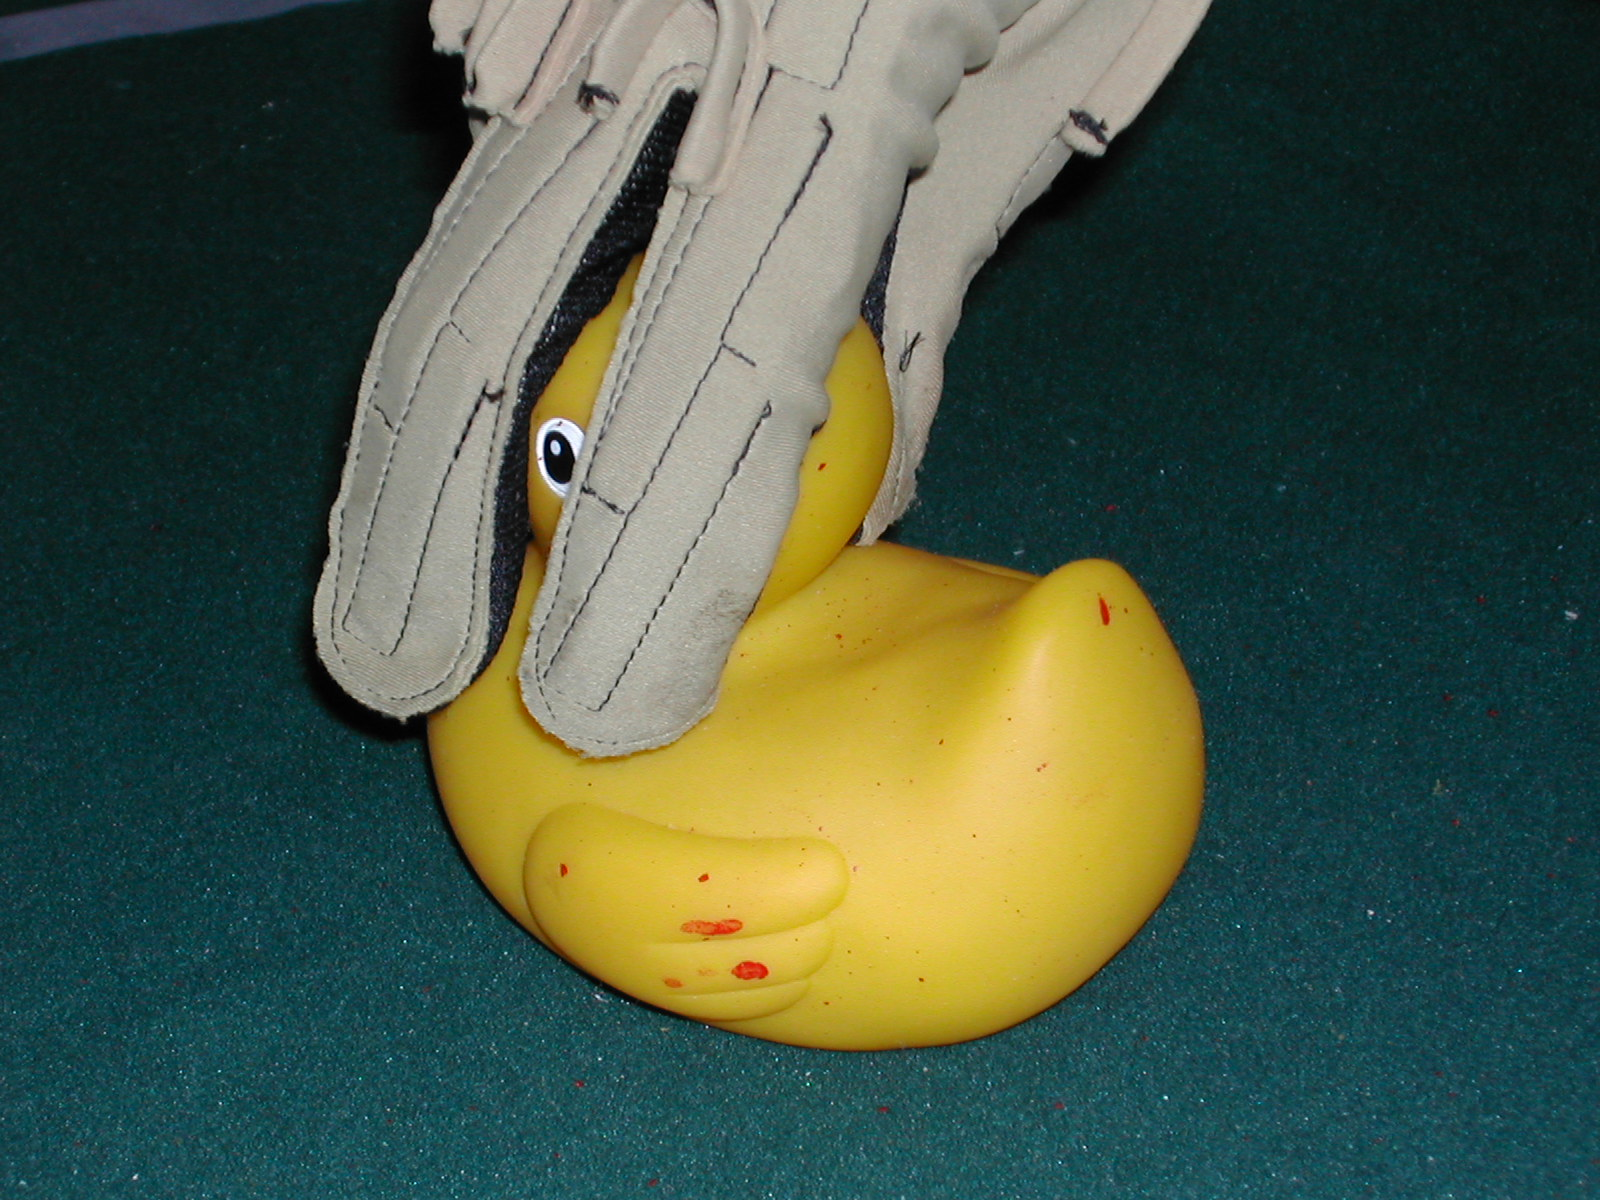
\includegraphics[height=0.08\textheight]{figs/grasping/grasp3.jpg}
      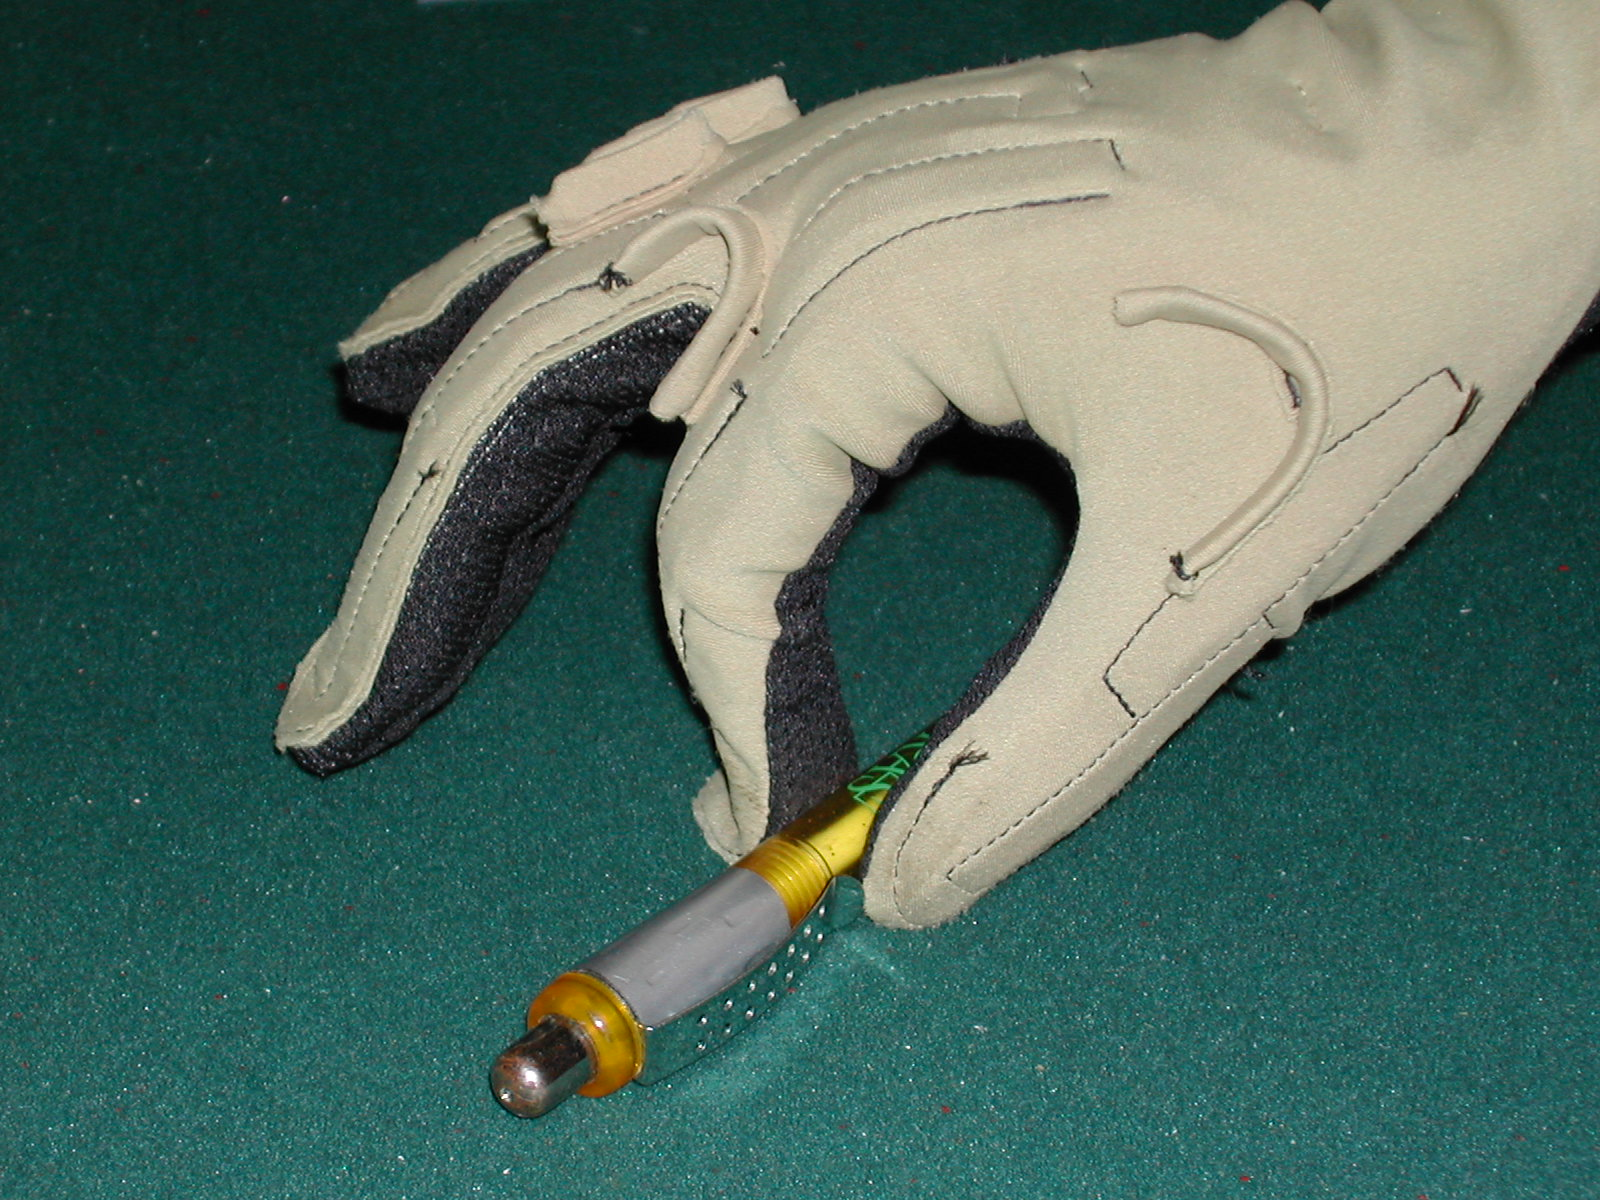
\includegraphics[height=0.08\textheight]{figs/grasping/grasp4.jpg}
      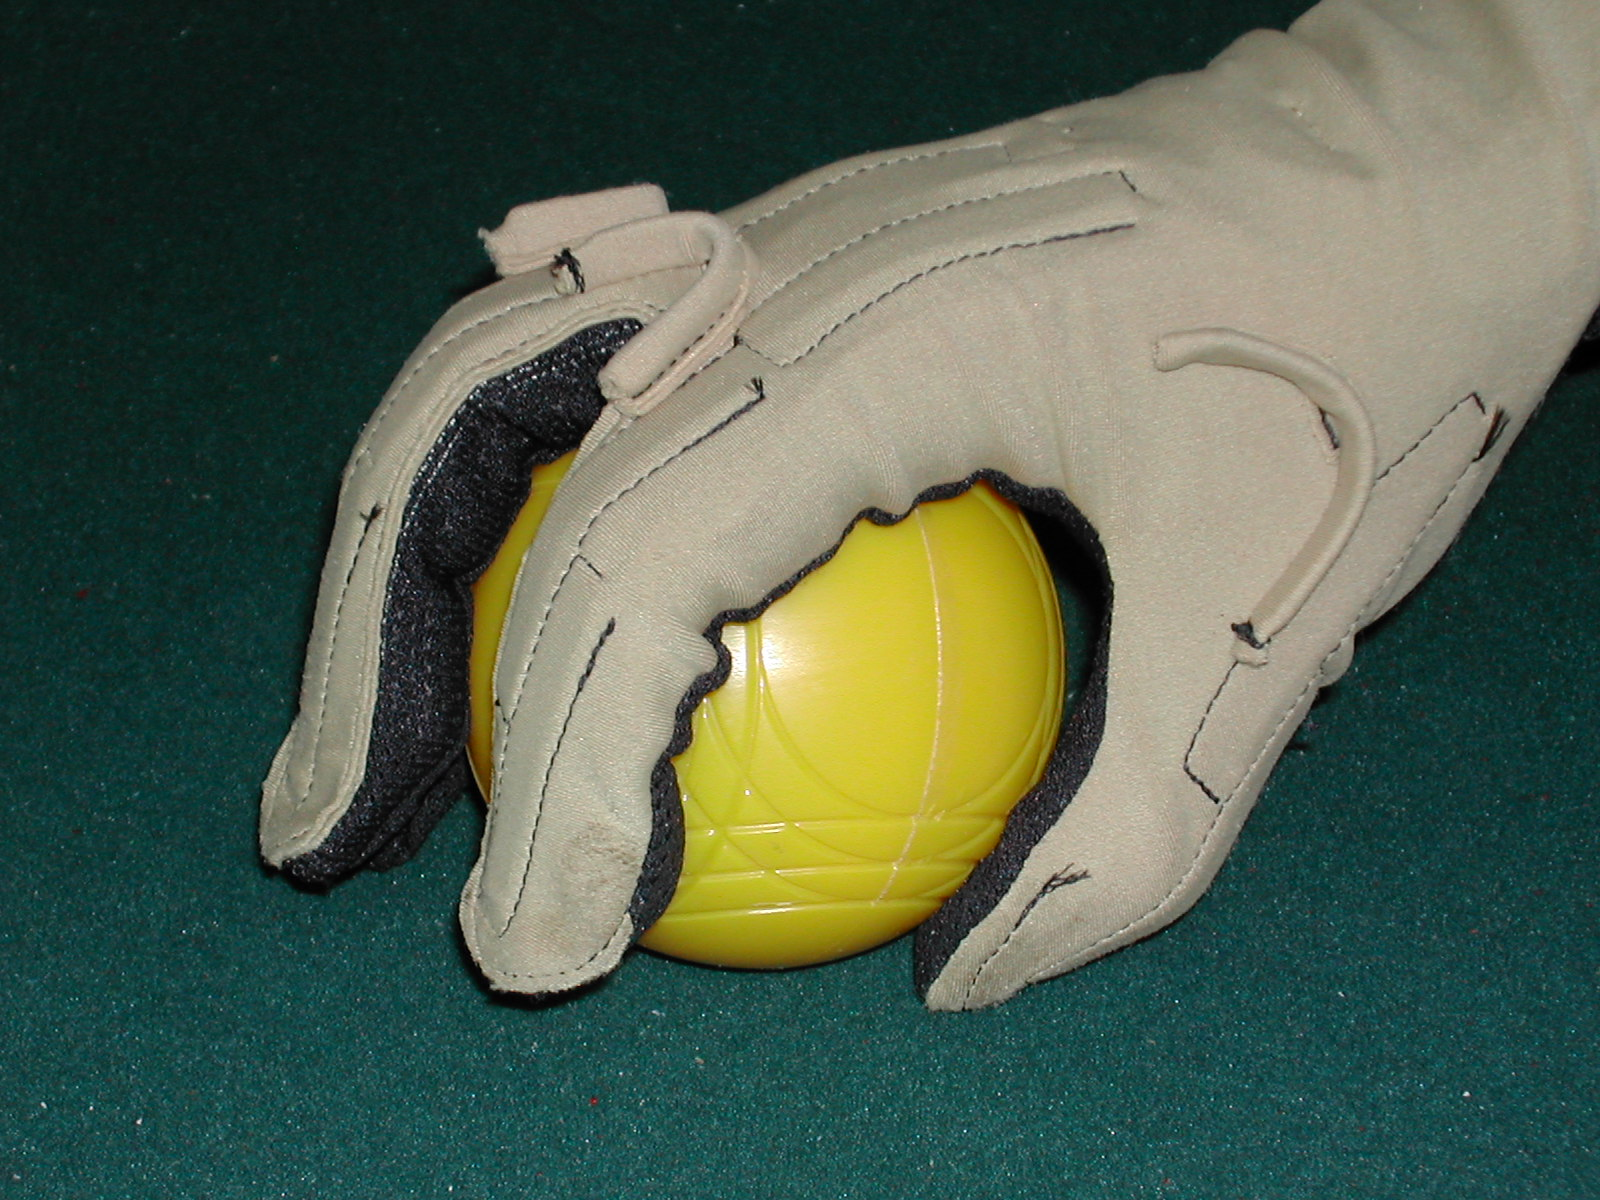
\includegraphics[height=0.08\textheight]{figs/grasping/grasp5.jpg} \\
    \end{tabular}
    \caption{(above) The devices and some of the objects used for the experiment,
    left to right: the CyberGlove, the Force Resistor Sensor attached
    to the subject's thumb, the beer can, the duct tape roll and the
    mug. (below) The $5$ grasp types to be recognized, left to right:
    power large, power flat, tripodal precision, thumb/index precision
    and spherical precision.}
    \label{fig:devices}
  \end{center}
\end{figure*}

%% The CyberGlove returns $22$ $8$-bit numbers linearly related to the
%% angles of the subject's hand joints; the sensors are embedded in the
%% glove in order for them to be adherent to the subject's skin. The
%% resolution of the sensors is on average about $0.5$ degree
%% \cite{cyberglove}, but the noise associated with the sensors has been
%% experimentally determined to be $1.1$ on average and $3$ at the
%% maximum \cite{212431}. The sensors describe the position of the three
%% phalanxes of each finger (for the thumb, rotation and two phalanxes),
%% the four finger-to-finger abductions, the palm arch, the wrist pitch
%% and the wrist yaw.

%% The FSR returns a $32$-bit number inversely related to the pressure
%% applied to the surface of the sensor. We used it as an on-off
%% indicator of when the subject was actually holding an
%% object. Toghether, the CyberGlove and FSR would give us a precise idea
%% of what the subject's hand posture was when grasping. All data were
%% collected, synchronised, and saved in real time at a frequency of
%% $50$Hz.

%% We then collected a number of objects encountered in everyday life,
%% and split them among $5$ pairs of sets, each set containing objects of
%% various size, colour, shape and affordances \cite{gibson}. The idea is
%% that each pair of sets would be associated with a particular type of
%% grasp, as identified by \cite{cutkosky}. The grasp types and
%% associated pairs were:

%% \begin{enumerate}
%%   \item \emph{power large grasp:} a beer can, a bottle and a box (set
%%     $1$); an anatomical hand model, a wooden toy dragon and a mug (set
%%     $2$);

%%   \item \emph{power flat grasp:} a hammer and a long Lego block (set
%%     $1$); a stapler, a screwdriver and and a TV remote control (set
%%     $2$);

%%   \item \emph{tripodal precision grip:} a small and a large ball, a
%%     rubber duck and a beer can (set $1$); a marker, a ballpoint pen
%%     and a ball (set $2$);

%%   \item \emph{thumb/index precision grip:} a knife, a duct tape roll,
%%     a short Lego block and a rubber duck (set $1$); a marker and a
%%     ballpoint pen (set $2$);

%%   \item \emph{spherical precision grip:} a small and a large ball and a
%%     rubber duck (set $1$); a fluffy toy airplane, a ball and a mug (set
%%     $2$).

%% \end{enumerate}

A number of objects encountered in everyday life were presented to the
subjects, who would then repeatedly grasp them in a particular way. The
grasp types were selected among those identified by Cutkosky in
\cite{cutkosky}: power large grasp, power flat grasp, tripodal
precision grip, thumb/index precision grip and spherical precision
grip. Figure \ref{fig:devices} shows three of the objects used in the
experiment and five examples of grasp types. Note that each object may
afford several grasp types, e.g., a rubber duck can be grasped either
via a tripodal precision grip, a thumb/index precision grip and/or a
spherical precision grip.

%% The experiment consisted of two phases. During the first phase, for
%% each pair, the first set of objects was put on the workspace, and the
%% subject was asked to choose one of the objects, grasp it with the
%% right hand, lift it and then put it back on the workspace. We
%% explicitly asked the subject to grasp \emph{using the grasp type
%% associated to the objects on the workspace}. We collected $60$ grasps
%% for each set of objects, resulting in $300$ grasps per subject,
%% divided by grasp type. During the second phase, we repeated the same
%% procedure but on a different day and using the second set of each
%% pair. Therefore, we would obtain analogous results to the first phase,
%% but allowing the subject to grasp different objects with the same
%% grasp type, and leaving a long time in between, in order for the
%% subject not to get used to a particular grasp type. Each phase was
%% completed by the subjects in $17$ to $18$ minutes.

%% In the end, this would allow us to gather $120$ grasps per grasp type
%% and subject; this means $960$ grasps per grasp type (for a total of
%% $4800$ grasps, since we had $5$ grasp types), well distributed across
%% various subjects, times of the day, fatigue conditions and objects.

%% The actual grasps, which would build the SVM training set, were
%% detected as follows: we found each interval of time during which the
%% FSR would signal contact, and then we took the CyberGlove sensors
%% values in the middle of the interval. We assumed that the hand posture would
%% not sensibly change during the grasping act, that is, while the subject
%% was lifting the object. Spurious grasp detections were removed from
%% the sample set, resulting in a total of $4512$ samples.

Each grasp is determined by the CyberGlove, therefore the input space
is $\RR^{22}$; and five categories, each corresponding to a grasp
type, were set up. The optimal hyperparameters $C$ and $\sigma$ were
found via grid search and cross-validation, as is customary.
%% The
%% machines were trained on data gathered during the first phase and
%% tested on data gathered during the second phase, and then
%% vice-versa. This way, the system was always tested on data related to
%% objects different from those seen during training, in order to remove
%% the possibility to learn the exact configuration of the hand rather
%% than the type of grasp.
We have compared OISVM with the batch method LIBSVM2 and the fixed-partition
technique. As in the experiments on place recognition experiments,
we have splitted the training data in several batches, to be able to use
the fixed partition method. In particular, in each training step we feed to
the systems all the data coming from an user.
A Gaussian kernel and three
different values of $\eta$ were used for OISVM. The results are shown
in Figure \ref{fig:exp:grasp}.

\begin{figure*}[t]
  \centering \footnotesize
  \begin{tabular}{c@{\hspace{0.5cm}}c}
    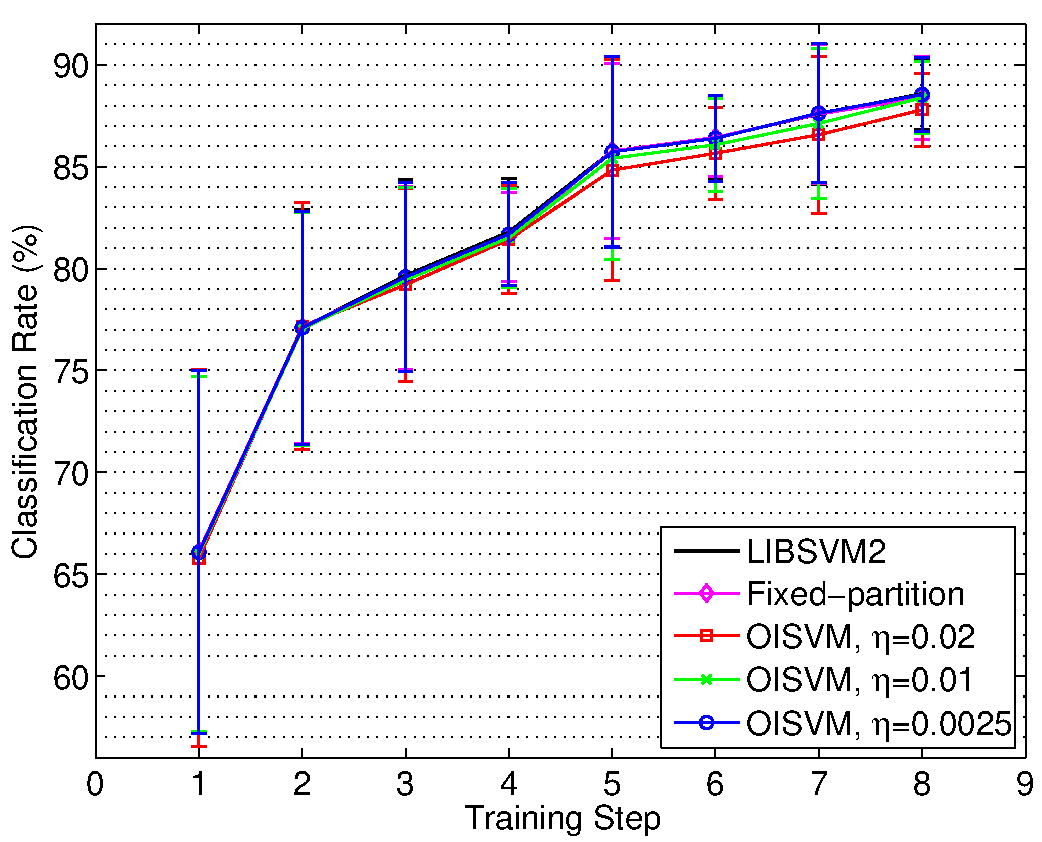
\includegraphics[width=0.47\linewidth]{figs/results/grasp_cr} &
    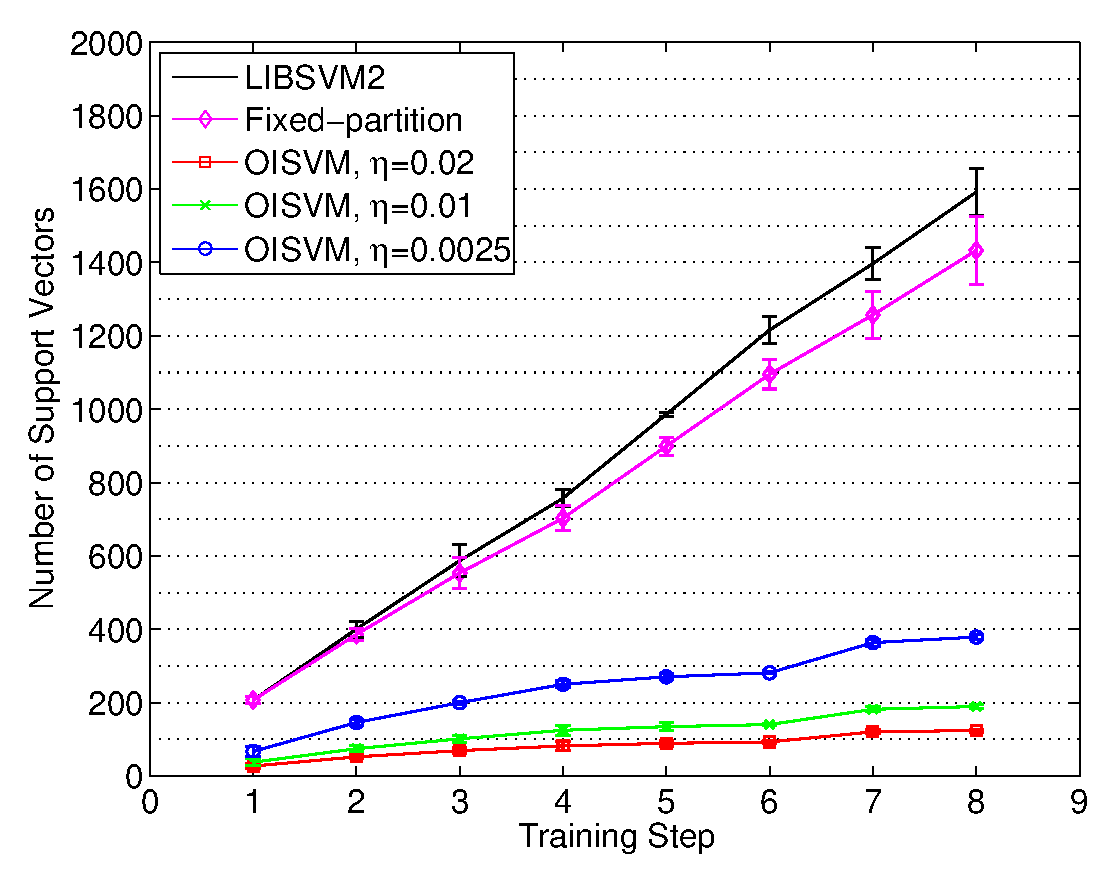
\includegraphics[width=0.47\linewidth]{figs/results/grasp_sv}
  \end{tabular}
  \caption{Classification rate (left) and average number of support
  vectors (left) for the grasping classification experiment. OISVM
  uses a Gaussian kernel and three different values of $\eta$.}
  \label{fig:exp:grasp}
\end{figure*}

Consider the Figure \ref{fig:exp:grasp}, left panel: it is apparent that the
classification rate is basically the same, uniformly and for all
approaches tested. The right panel shows that, in agreement with the
previous experiments, LIBSVM2 and the fixed partition method gather a
number of SVs which grows proportionally with the training set. On the
other hand, OISVM with various values of $\eta$ uniformly show a
dramatically smaller number of SVs, getting to as few as $124$ SVs in
the case for $\eta=0.02$, losing only $0.8\%$ of accuracy compared to
LIBSVM2.


\section{Conclusions}
\label{sec:conclusions}
In this paper we have presented, implemented and tested a novel system
for on-line learning based upon Support Vector Machines. The method,
On-line Independent SVMs (OISVMs), avoids using in the solution those
support vectors which are linearly dependent of previous ones in the
feature space; linear independence is checked incrementally every time
a new sample is made available to the system; the optimization problem
is solved via an incremental algorithm which benefits of the small size
of the basis set. A parameter called $\eta$ is employed to trade
better/worse accuracy for more/fewer support vectors in the basis.

We tested the method both on a standard set of benchmark databases and
on two real-world case studies, namely: $(a)$ place recognition in an
indoor environment and $(b)$ human grasping classification. Both
real-world experiments have been carefully crafted in order to take
into account changing conditions in the environment: robot images were
acquired under different weather conditions and across a time span of
several months; grasping was done across a time span of several days,
with several different objects and by several human subjects with
little or no prior knowledge about the experiment.

The experimental results, carried out for various values of $\eta$,
show that OISVMs enjoy an excellent accuracy/basis size trade
off. Moreover, a deeper analysis of the value of the objective
function at the end of the training reveals that our method
selects the basis vectors in such a way as to better minimize
it.

%% %In particular, in the case of
%% %robot localisation, we can reduce the number of SVs up to $4.5$ times
%% %with a negligeble loss in performance; whereas, in grasping classification
%% %we can reduce more than $13$ times.
%% Furthermore, our analysis clearly shows that OISVMs improve on SVMs,
%% proving to be highly adaptive to environmental changes (Introduction,
%% requirement $1$) and accurate (Introduction, requirement $2$), by
%% keeping the number of support vectors extremely small, thus minimizing
%% the need for storage and making testing and training significantly
%% faster (Introduction, requirements $3$ and $4$).

An open issue is how to choose $\eta$ to achieve an optimal trade-off
between accuracy and speed for a given task. Both theory and experiments
clearly point out the relevance of $\eta$ for fully exploiting the power of
OISVMs, but its choice is today one of the heuristics of the method, along with
the choice of $C$, the kernel function and the kernel parameters. Therefore,
the only solution we can point to the reader is the use of a validation set,
as it is customary for the other previously mentioned SVM parameters.
How to determine $\eta$ in a more principled way will be the focus of future
work.

Another research direction we plan to pursue is to extend the method so to
handle an underlying dynamic distribution of the data, as opposed to the static
scenario considered in this paper. This problem has been already tackled in 
generative frameworks (i.e. \cite{YoonRDG08}) but it is still far from being solved
in discriminative settings.

Lastly we plan to use OISVM in a life-long learning scenario. So far OISVMs are
able to perform continuous learning on data collected on a span of
time of up to several months, but it is still not possible to use them
with a truly never-ending stream of data, since all training samples
must anyway be retained. To achieve this goal we plan to extend
the method so to include a forgetting mechanism.
%%  Another important
%% issue is multimodality: systems typically acquire
%% inputs from different modalities that must be combined together during
%% learning so to build a rich internal model. Thus, we plan to extend
%% OISVMs so to work on multimodal data streams.
%Also, so far we have considered a purely supervised learning
%framework, but while it is reasonable to have a privileged teacher for
%some time, in general the system will have to act autonomously. Thus,
%OISVMs should be extended to the semi-supervised framework. Future
%work will address these issues.


\section*{Acknowledgments}
Thanks to Joseph Keshet for helping improving the manuscript.
This work was supported by EU projects RobotCub (IST-2004-004370),
NEURObotics (FP6-IST-001917) and DIRAC (FP6-0027787).

{\small
\bibliographystyle{IEEEtran}
\bibliography{paper}
}

\end{document}
